\phantomsection
\chapter[Comparing Two Viral Spike Proteins]{Comparing Two Viral Spike Proteins\chapsubhead{with Chris Lee}}
\label{chapter:coronavirus_2}
\renewcommand{\chaptertitle}{Comparing Two Viral Spike Proteins}
\addcontentsline{cc}{chapter}{Chapter \thechapter} % Adds chapter number to table of contents

\FloatBarrier
\phantomsection

\section{Part 2: Finding Local Differences in Protein Structures with Qres}
\label{sec:multiseq}
\phantomsection

In part 1, we used a variety of existing software resources to predict the structure of the SARS-CoV-2 spike protein from its amino acid sequence. We then discussed how to compare our predicted structures against the experimentally confirmed structure of the protein.

Now begins part 2, in which we examine how the structure of the SARS-CoV-2 spike protein compares against the SARS-CoV spike protein. In keeping with the biological maxim that the \textit{structure} of a protein informs the \textit{function} of that protein, can we find any clues lurking in the spike proteins' structure that would indicate why the two viruses had different fates?

\FloatBarrier
\phantomsection
\subsection{Focusing on a variable region of interest in the spike protein}

In part 1, we saw that the spike protein is much more variable than other regions of the viral genomes. We even see variable and conserved regions within the spike protein, as \autoref{fig:spike_protein_similarity} indicates.

The most variable region between the two viruses in the spike protein is the \textdefnogloss{receptor binding motif (RBM)}, part of the receptor binding domain (RBD) whose structure we predicted using GalaxyWEB. The RBM is the component of the RBD that mediates contact with ACE2.

The fact that the region binding to the target human enzyme has mutated so much makes it a fascinating region of study. Do the mutations that SARS-CoV-2 has accumulated somehow make it easier for the virus to infect human cells?

As we hone in on the RBM, \autoref{fig:RBM_alignment} shows an alignment of the 70 amino acid long RBM region from SARS-CoV and SARS-CoV-2.\\

\begin{figure}[h]
	\centering
	\mySfFamily
	
\includegraphics[width = 0.7\textwidth]{../images/RBM_alignment.png}
	\caption{An alignment of the RBM of the human SARS-CoV virus (first row) and the SARS-CoV-2 virus (second row). Amino acids that are highlighted in green represents matches between the two sequence. Beneath each column is the conservation between the two sequences, where full conservation indicates a match and partial conservation indicates a mismatch.}
	\label{fig:RBM_alignment}
\end{figure}

We know from our work in structure prediction that just because the sequence of a protein has been greatly mutated does not mean that the structure of that protein has changed much. Therefore, in this section, we will start a structural comparison of the SARS-CoV and SARS-CoV-2 spike proteins. All of this analysis will be performed using the software resources ProDy and VMD.

\FloatBarrier
\phantomsection
\subsection{Using bound spike-ACE2 enzymes}

In addition to verifying the structure of the spike protein in both SARS-CoV and SARS-CoV-2, researchers also determined the structure of the RBD complexed with ACE2 in both SARS-CoV (PDB entry: \href{https://www.rcsb.org/structure/2ajf}{2ajf}) and SARS-CoV-2 (PDB entry: \href{https://www.rcsb.org/structure/6vw1}{6vw1}).\\

\begin{note}[%
	The experimentally verified SARS-CoV-2 structure is a \textit{chimeric} protein formed of the SARS-CoV RBD in which the RBM has the sequence from SARS-CoV-2. A chimeric RBD was used for complex technical reasons to ensure that the crystallization process during X-ray crystallography could be borrowed from that used for SARS-CoV.
	]\end{note}

Because we know the structures of the bound complexes, we can produce 3-D visualizations of the two different complexes and look for structural differences involving the RBM. We will use VMD to produce this visualization, rotating the structures around to examine potential differences. However, we should be wary of only trusting our eyes to guide us; can we use a computational approach to tell us where to look for structural differences between the two RBMs?

\FloatBarrier
\phantomsection
\subsection{A first attempt at identifying local dissimilarities between protein structures}

To assess the accuracy of a predicted structure in \autoref{chapter:coronavirus_1}, we introduced a metric called root mean square deviation (RMSD) for quantifying the difference between two protein structures. RMSD offered an excellent method for a \textit{global} comparison (i.e., a comparison across all structures), but we are interested in the \textit{local} regions where the SARS-CoV and SARS-CoV-2 complexes differ. To this end, we will need an approach that considers individual amino acids in similar protein structures.\\

\begin{qbox}[%
	How could we compare individual amino acid differences of two protein structures?
	]\end{qbox}

Recall the following definition of RMSD for two protein structures \textvar{s} and \textvar{t}, in which each structure is represented by the positions of its \textvar{n} alpha carbons $(s_{1}, \cdots, s_{n})$ and $(t_{1}, \cdots, t_{n})$:

\begin{center}
$\text{RMSD}(s, t) = \sqrt{\dfrac{1}{n} \cdot (d(s_1, t_1)^2 + d(s_2, t_2)^2 + \cdots + d(s_n, t_n)^2)}$\,.
\end{center}

\noindent If two similar protein structures differ in a few locations, then the corresponding alpha carbon distances $d(s_{i}, t_{i})$ will likely be higher at these locations. However, we will introduce a more sophisticated approach for
comparing the local structure of $s_{i}$ against $t_{i}$. First, however, we will discuss an alternative to RMSD for computing global structure.

\FloatBarrier
\phantomsection
\subsection{Contact maps and Qres}

One of the weaknesses of RMSD that we pointed out in part 1 is that a change to a single bond angle at the \textvar{i}-th position may cause $d(s_{j}, t_{j})$ to be nonzero when $j > i$, even though the structure of the protein downstream of this bond angle has not changed. For example, recall \autoref{fig:RMSD_weakness_mutation} from our discussion of the Kabsch algorithm, in which we showed two toy protein structures that are identical except for a single bond angle. All of the alpha carbon distances $d(s_{i}, t_{i})$ for \textvar{i} at least equal to 4 will be thrown off by this changed angle. These structures are reproduced in \autoref{fig:single_bond_angle}.\\

\begin{figure}[h]
	\centering
	\mySfFamily
	\includegraphics[width = 0.7\textwidth]{../images/single_bond_angle.png}
	\caption{Two toy protein structures in which the bond angle between the third and fourth alpha carbon has been changed. This change does not affect the distance between the \textvar{i}-th and \textvar{j}-th alpha carbons when \textvar{i} and \textvar{j} are both at least equal to 4.}
	\label{fig:single_bond_angle}
\end{figure}

However, note in \autoref{fig:single_bond_angle} that when \textvar{i} and \textvar{j} are both at least equal to 4, the distance $d(s_{i}, s_{j})$ between the \textvar{i}-th and \textvar{j}-th alpha carbons in \textvar{S} will still be similar to the distance $d(t_{i}, t_{j})$ between the same alpha carbons in \textvar{T}. This observation leads us to a more robust approach for measuring differences in two protein structures, which compares \textvar{all} pairwise distances $d(s_{i}, s_{j})$ in one protein structure against the corresponding distances $d(t_{i}, t_{j})$ in the other structure.

To help us visualize all these pairwise distances, we will introduce the \textdef{contact map}{contact map}{a binary matrix used to determine which pairs of alpha carbons in two proteins are close to each other} of a protein structure, which is a binary matrix indicating whether two alpha carbons are near each other. After setting a threshold distance, for a given structure \textvar{s}, we set $M(i, j) = 1$ if the distance $d(s_{i}, s_{j})$ is less than the threshold, and $M(i, j) = 0$ if $d(s_{i}, s_{j})$ is greater than or equal to the threshold.

\autoref{fig:Contact} shows the contact maps for the SARS-CoV-2 and SARS-CoV spike proteins (both full proteins and single chains) with a threshold distance of twenty angstroms. In this map, we color contact map values black if they are equal to 1 (close amino acid pairs) and white if they are equal to 0 (distant amino acid pairs).

We note two things in the contact maps in \autoref{fig:Contact}. First, many black values cluster around the main diagonal of the matrix, since amino acids that are nearby in the protein sequence will remain near each other in the 3-D structure. Second, the contact maps for the two proteins are very similar, reinforcing that the two proteins have similar structures.\\

\begin{figure}[h]
	\centering
	\mySfFamily
	\includegraphics[width = 0.8\textwidth]{../images/Contact.png}
	\caption{The contact maps of the SARS-CoV-2 spike protein (top left), SARS-CoV spike protein (top right), single chain of the SARS-CoV-2 spike protein (bottom left), and single chain of the SARS-CoV spike protein (bottom right). If the distance between the \textvar{i}-th and \textvar{j}-th amino acids in a protein structure is 20 angstroms or less, then the (\textvar{i}, \textvar{j})-th cell of the figure is colored black. The SARS-CoV-2 and SARS spike proteins have very similar contact maps, indicating similar global structures.}
	\label{fig:Contact}
\end{figure}

\begin{note}[%
	Interested in learning how to make contact maps? We will use ProDy to do so in a later tutorial.
	]\end{note}

\begin{qbox}[%
	How do you think the contact map will change as we increase or decrease the threshold distance?
	]\end{qbox}

We obtain some insight into how two proteins differ structurally at the \textvar{i}-th amino acid if we look at all of the \textvar{i}-th row's values; that is, if we compare all of the $d(s_{i}, s_{j})$ values to all of the $d(t_{i}, t_{j})$ values.

We will use pairwise distances between alpha carbons to determine how different two proteins are at the \textvar{i}-th alpha carbon, using a metric called \textdefnogloss{Q per residue (Qres)}.  The formal definition of Qres for two structures \textvar{s} and \textvar{t} having \textvar{N} residues is

\begin{center}
$Q_{\text{res}}^{(i)} = \dfrac{1}{N-k} \displaystyle \sum^{\text{residues}}_{j\neq i-1,i,i+1} \exp\left[-\dfrac{[d(s_i,s_j)-d(t_i,t_j)]^2}{2\sigma^2_{i,j}}\right]$\,.
\end{center}

\noindent In this equation, $\exp(x)$ means $e^{x}$. This equation also includes the following parameters.

\begin{itemize}
	\item \textvar{k} is equal to 2 at either the start or the end of the protein (i.e., \textvar{i} is equal to 1 or \textvar{N}), and \textvar{k} is equal to 3 otherwise.
	\item The variance term $\sigma_{ij}^2$ is equal to $\left\lvert{i-j}\right\rvert ^{0.15}$, which corresponds to the sequence separation between the \textvar{i}-th and \textvar{j}-th alpha carbons.
\end{itemize}

\begin{note}[%
	The above definition assumes that the two proteins have the same length or have been pre-processed by removing amino acids that only occur in one protein. Generalizations of Qres for proteins of non-equal length exist that first align proteins and retain only those amino acids for structural comparison that are shared by the two proteins.
	]\end{note}

If two proteins are very similar at the \textvar{i}-th alpha carbon, then for every \textvar{j}, $d(s_{i}, s_{j}) - d(t_{i}, t_{j})$ will be close to zero, making term inside the summation in the Qres equation will be close to 1. The sum will be equal to approximately $N - k$, and so Qres will be close to 1. As two proteins become more different at the \textvar{i}-th alpha carbon, then the term inside the summation will head toward zero, and so will the Qres value as well.

As a result, we think of Qres as a similarity metric ranging between 0 and 1, with low scores representing low similarity between two proteins at the \textvar{i}-th position, and higher scores representing high similarity at this position.

We now will compute Qres for the SARS-CoV and SARS-CoV-2 spike proteins using the VMD plugin \href{https://bit.ly/3LwTYmp}{\textdefnogloss{Multiseq}}, a bioinformatics analysis environment. After determining Qres, we will visualize the individual locations where the two RBD regions differ. \tutorial[coronavirus/tutorial_multiseq]

\FloatBarrier
\phantomsection
\subsection{Local comparison of spike proteins leads us to a region of interest}

By computing Qres at every position of the two coronavirus RBD regions, we can form a ``structural'' alignment of the two regions (\autoref{fig:QresResult} (top)). Blue columns correspond to amino acids with high Qres (meaning high structural similarity), and red columns correspond to amino acids with low Qres (meaning low structural similarity).

If we zoom in on the region around position 150 of the alignment, we find a 13-column region of the alignment within the RBD region for which Qres values are significantly lower than they are elsewhere. This region corresponds to positions 476 to 485 in the SARS-CoV-2 spike protein (\autoref{fig:QresResult} (bottom)).\\

\begin{figure}[h]
	\centering
	\tabcolsep = 1em
	\mySfFamily
	\begin{tabular}{c}
		\includegraphics[width = 0.9\textwidth]{../images/QresResult.png} \\
		\includegraphics[width = 0.4\textwidth]{../images/QresResult_cropped.png} \\
	\end{tabular}
	\caption{(Top) A snapshot of the sequence alignment between the SARS-CoV RBD (first row) and the SARS-CoV-2 chimeric RBD (second row). Columns are colored along a spectrum from blue (high Qres) to red (low Qres), with positions that correspond to an inserted or deleted amino acid colored red. (Bottom) A region of the alignment with low Qres, which corresponds to amino acids at positions 476 to 485 in the SARS-CoV-2 spike protein.}
	\label{fig:QresResult}
\end{figure}

We also can create a 3-D visualization of the structures. \autoref{fig:QresVMD} shows the superimposed structures of both the SARS and SARS-CoV-2 RBD bound with ACE2, shown in green. The same color-coding of columns of the multiple alignment in \autoref{fig:QresResult} is used to highlight differences between the SARS-CoV and SARS-CoV-2 structures. The low-Qres region of the RBM alignment that we highlighted in \autoref{fig:QresResult} is outlined in \autoref{fig:QresVMD}.\\

\begin{figure}[h]
	\centering
	\mySfFamily
	\includegraphics[width = 0.7\textwidth]{../images/QresVMD.png}
	\caption{A visualization showing the superposed structures of SARS-CoV-2 chimeric RBD (Shang et al. 2020) and SARS RBD in blue and red based on Qres. Blue indicates regions of high Qres, and red indicates regions of low Qres. ACE2 is shown in green. The highlighted region corresponds to the part of the RBM with a potential structural difference. Because it is adjacent to ACE2, it is likely that the structural difference here will affect ACE2 interactions.}
	\label{fig:QresVMD}
\end{figure}

\begin{note}[%
	Although the rest of the proteins are similar, there are other parts of the RBD at the top of the protein that show dissimilarities in the two proteins, which may be attributable to an experimental artifact. The authors of the work in which the comparison was published have pointed out that the highlighted region is unlikely to be an artifact of the experimentation because it is ``buried at the RBD–ACE2 interface and did not affect crystallization''.
	]\end{note}

Finding this highlighted region in the RBM where the structures of the SARS-CoV and SARS-CoV-2 spike proteins differ is an exciting development. We will next explore this region of the protein structure to determine whether the mutations acquired by SARS-CoV-2 may have influenced the binding affinity of the virus spike protein with the human ACE2 enzyme.\\

\FloatBarrier
\phantomsection

\section{Analysis of Structural Protein Differences}
\label{sec:structural_differences}
\phantomsection
\subsection{Visualizing a region of structural differences}

In \autoref{sec:multiseq}, we identified a region between residues 476 and 485 of the SARS-CoV-2 spike protein that corresponds to a structural difference between the SARS-CoV-2 and SARS-CoV RBMs. We now wish to determine whether the differences we have found affect binding affinity with the human ACE2 enzyme.

We know from our work in this course that a tiny change can produce a big difference in the high-level behavior of a finely tuned system. It may therefore be the case that subtle changes in the ability of SARS-CoV-2 to stick to the ACE2 enzyme can change the virus's infectiousness enough to greatly influence its spread through the human population.

We will first use VMD to highlight the amino acids in the region of interest of the SARS-CoV-2 spike protein's structure. \tutorial[coronavirus/tutorial_visualization]

\FloatBarrier
\phantomsection
\subsection{Analyzing three sites of conformational differences}

Shang et al. 2020 identified three sites showing significant conformational differences between the SARS-CoV-2 and SARS-CoV spike proteins. We will discuss each of these three locations and see how they affect binding affinity between the spike protein and ACE2.

\FloatBarrier
\phantomsection
\subsection{Site 1: loop in ACE2-binding ridge}

The first location is our region of interest from the previous section and is found on a loop in a region called the ACE2 binding ridge. This region is shown in \autoref{fig:Ridge}, in which SARS-CoV-2 is on left and SARS-CoV is on the right.

Structural differences are challenging to show with a 2-D image, and we encourage you to use VMD to view the 3-D representation of the protein. \tutorial[coronavirus/tutorial_multiseq]\\

\begin{qbox}[%
	See if you can identify the major structural difference between the proteins in \autoref{fig:Ridge}. Hint: look at the yellow residue.
	]\end{qbox}

\begin{figure}[h]
	\centering
	\mySfFamily
	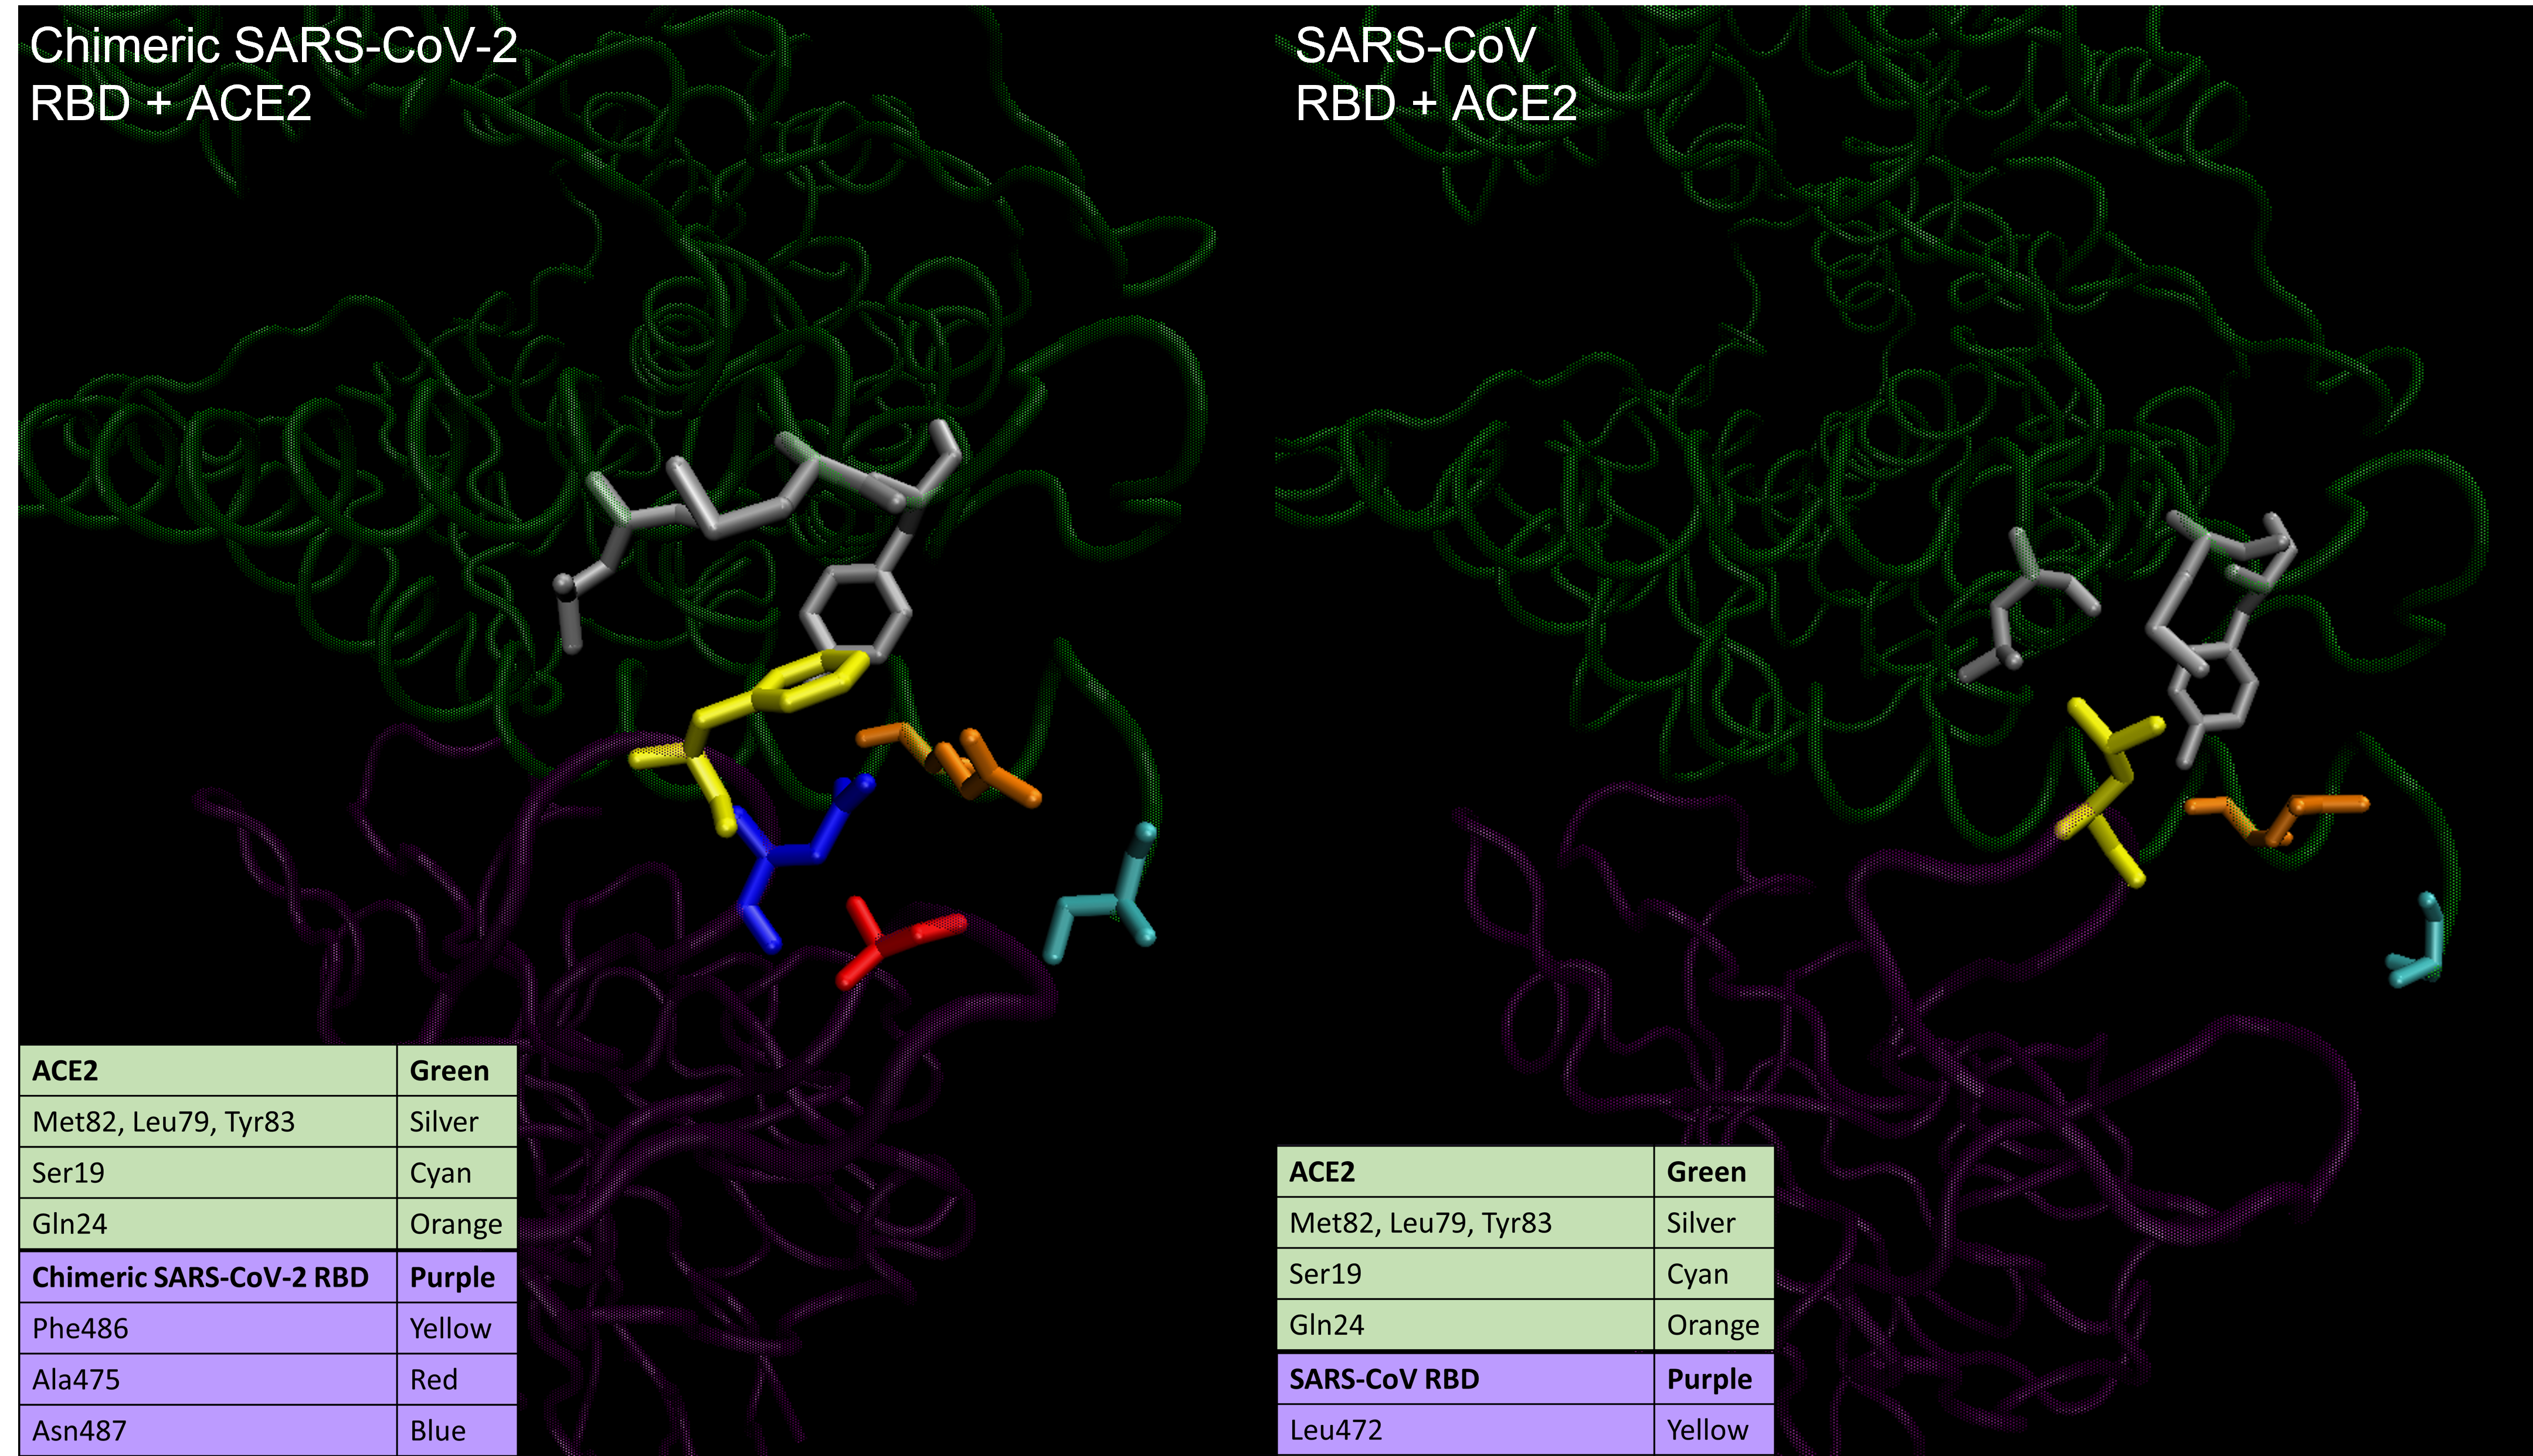
\includegraphics[width = 0.85\textwidth]{../images/Ridge.png}
	\caption{A visualization of the loop in the ACE2-binding ridge that is conformationally different between SARS-CoV-2 (left) and SARS-CoV (right). The coronavirus RBD is shown in purple, and ACE2 is shown in green. Structural differences cause certain amino acid residues (highlighted in various colors) to behave differently between the two interactions.}
	\label{fig:Ridge}
\end{figure}

The most noticeable difference between SARS-CoV-2 and SARS-CoV in this region relates to a ``hydrophobic pocket'' of three hydrophobic ACE2 residues at positions 82, 79, and 83 (methionine, leucine, and tyrosine). This pocket, which is colored silver in \autoref{fig:Ridge}, is hidden away from the outside of the ACE2 enzyme to keep these amino acids away from water. In SARS-CoV-2, the RBD phenylalanine residue at position 486 (yellow) inserts itself into the pocket, favorably interacting with ACE2. These interactions do not happen with SARS-CoV, and its corresponding RBD residue, a leucine at position 472 (yellow), is not inserted into the pocket.

In what follows, we use a three-letter identifier for an amino acid followed by a number to indicate the identity of that amino acid followed by its position within the protein sequence. For example, the phenylalanine at position 486 of the SARS-CoV-2 spike protein would be called Phe486.

Although the interaction with the hydrophobic pocket is the most critical difference between SARS-CoV-2 and SARS-CoV, we highlight two other key differences. First, in SARS-CoV-2, a main-chain hydrogen bond forms between Asn487 and Ala475 (shown in red in \autoref{fig:Ridge}), which creates a more compact ridge conformation, pushing the loop containing Ala475 closer to ACE2. This repositioning allows for the N-terminal residue Ser19 in ACE2 (colored cyan in \autoref{fig:Ridge}) to form a hydrogen bond with the main chain of Ala475. Second, Gln24 in ACE2 (colored orange in \autoref{fig:Ridge}) forms a new contact with the RBM.

\FloatBarrier
\phantomsection
\subsection{Site 2: hotspot 31}

\textbf{Hotspot 31} is not a failed Los Angeles nightclub but rather our second region of notable conformational differences between SARS-CoV-2 and SARS-CoV, which was studied in SARS-CoV as early as 2008. This location earns its name because it involves a salt bridge between Lys31 and Glu35. Hotspot 31 is colored red in \autoref{fig:Hotspot31}.\\

\begin{qbox}[%
	Once again, see if you can spot the differences between SARS-CoV-2 and SARS-CoV.
	]\end{qbox}

\begin{figure}[h]
	\centering
	\mySfFamily
	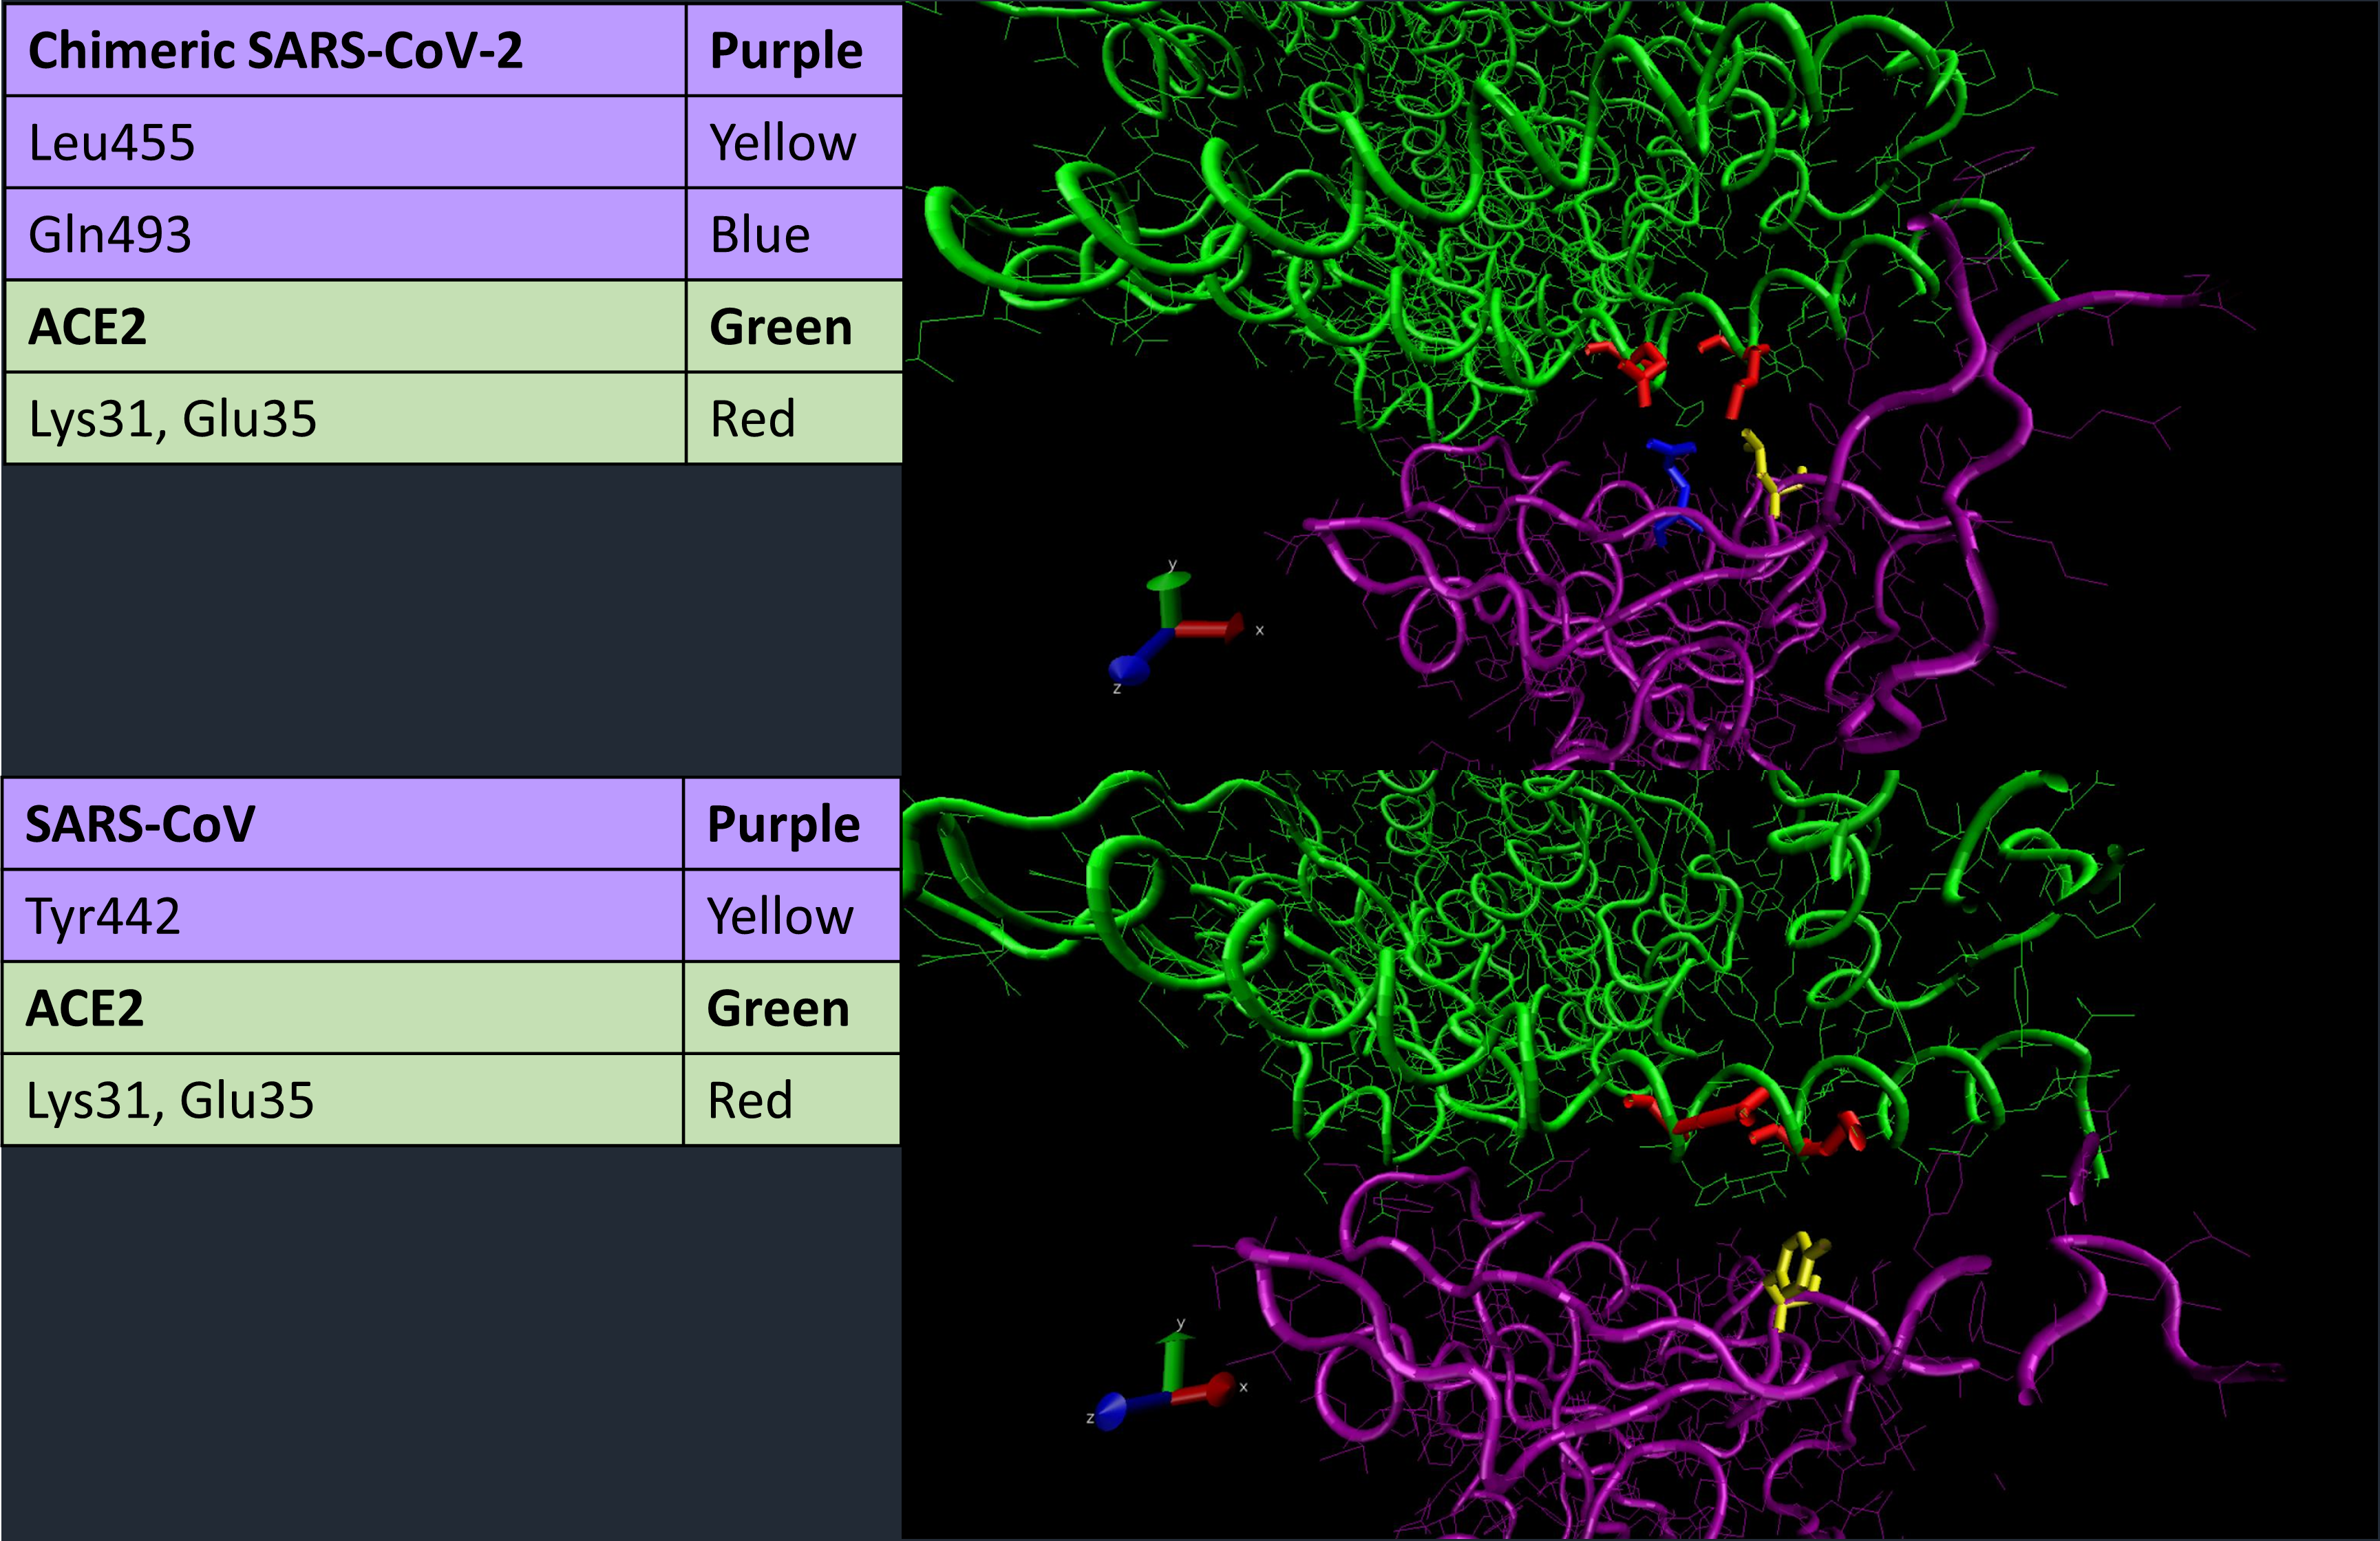
\includegraphics[width = 0.85\textwidth]{../images/Hotspot31.png}
	\caption{Visualizations of hotspot 31 in SARS-CoV-2 (left) and SARS-CoV (right). The RBD is shown in purple, and ACE2 is shown in green. In SARS-CoV, hotspot 31 corresponds to a salt bridge, which is broken in SARS-CoV-2 to form a new hydrogen bond.}
	\label{fig:Hotspot31}
\end{figure}

\autoref{fig:Hotspot31} shows how the salt bridge is radically different in the two viruses. In SARS-CoV, the two residues appear to point towards each other because in the SARS-CoV RBM, Tyr442 (colored yellow in right figure) supports the salt bridge between Lys31 and Glu35 on ACE2. In contrast to Tyr442 in SARS-CoV, the corresponding amino acid in SARS-CoV-2 is the less bulky Leu455 (colored yellow in left figure), which provides less support to Lys31. This causes the salt bridge to break, so that Lys31 and Glu35 in ACE2 point in parallel toward the RBD residue Gln493 (colored blue). This change allows Lys31 and Glu35 to form hydrogen bonds with Gln493 in SARS-CoV-2.

\FloatBarrier
\phantomsection
\subsection{Site 3: hotspot 353}

Finally, we consider \textbf{hotspot 353}, which involves another salt bridge connecting Lys353 and Asp38 in ACE2. In this region, the difference between the residues is so subtle that it takes a keen eye to notice them in \autoref{fig:Hotspot353}.

\begin{figure}[h]
	\centering
	\mySfFamily
	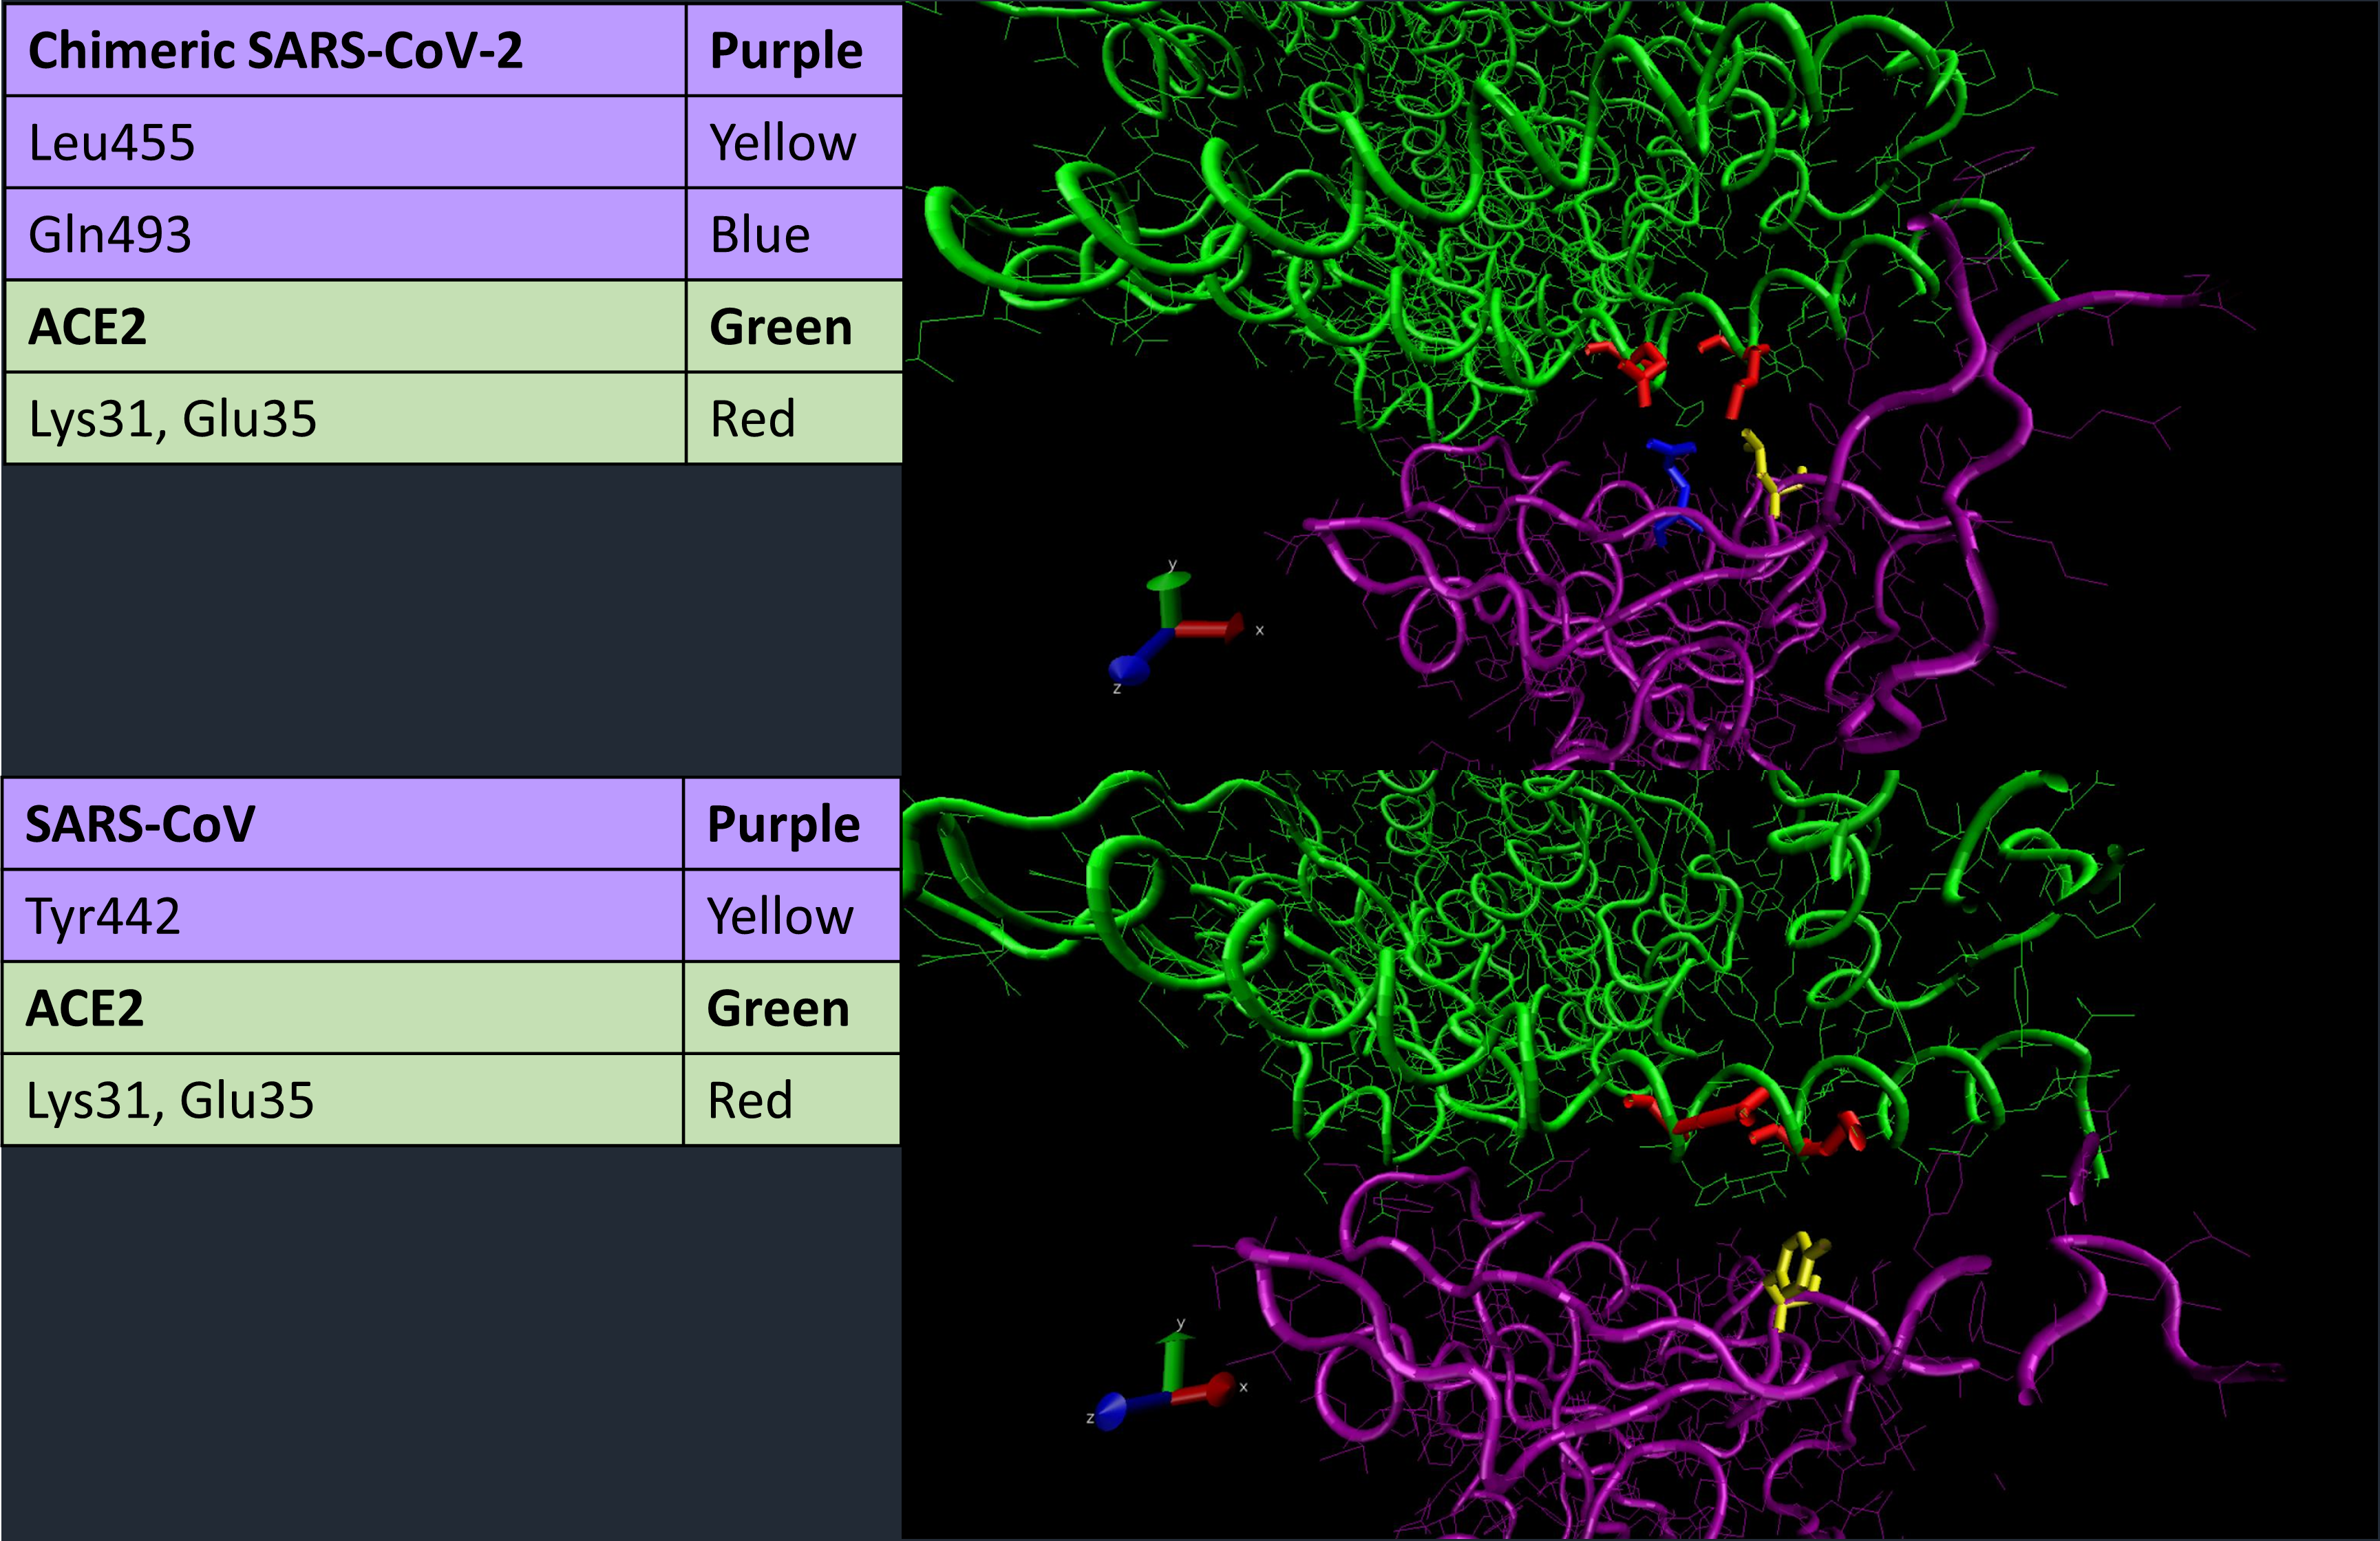
\includegraphics[width = 0.85\textwidth]{../images/Hotspot31.png}
	\caption{Visualizations of hotspot 353 in SARS-CoV-2 (left) and SARS-CoV (right). The RBD is shown in purple, and ACE2 is shown in green. In SARS-CoV, the RBD residue Thr487 (yellow) stabilizes the salt bridge between ACE2 residues Lys 353 and Asp38 (red). In SARS-CoV-2, the corresponding RBD residue Asn501 (yellow) provides less support, causing ACE2 residue Lys353 (red residue on the left) to be in a slightly different conformation and form a new hydrogen bond with the RBD.}
	\label{fig:Hotspot353}
\end{figure}

In SARS-CoV, the methyl group of Thr487 (colored yellow in \autoref{fig:Hotspot353} (right)) supports the salt bridge on ACE2, and the side-chain hydroxyl group of Thr487 forms a hydrogen bond with the RBM backbone. The corresponding SARS-CoV-2 amino acid Asn501 (colored yellow in left figure) also forms a hydrogen bond with the RBM main chain. However, similar to what happened in hotspot 31, Asn501 provides less support to the salt bridge, causing Lys353 on ACE2 (colored red) to be in a different conformation. This allows Lys353 to form an extra hydrogen bond with the main chain of the SARS-CoV-2 RBM while maintaining the salt bridge with Asp38 on ACE2.

You may be wondering how researchers can be so fastidious that they would notice all these subtle differences between the proteins, even if they know where to look. The fact is that they have help in their subjective descriptions of how protein structure affects binding. In the next section, we will discuss how to \textit{quantify} the improved binding of SARS-CoV-2 to ACE2 at the three locations described above.\\

\FloatBarrier
\phantomsection

\section{Quantification of Protein Interaction Energy}
\label{sec:interaction_energy}
\phantomsection
\subsection{Computing energy of a bound complex}

In part 1, we searched for the tertiary structure that best ``explains'' a protein's primary structure by looking for the structure with the lowest potential energy (i.e., the one that is the most chemically stable).

To quantify whether two molecules bind well, we will borrow this idea and compute the potential energy of the complex formed by the viral spike protein and ACE2. If two molecules bind well, then the complex will have a very low potential energy. In turn, if we compare the SARS-CoV-2 RBD-ACE2 complex against the SARS-CoV RBD-ACE2 complex, and we find that the potential energy of the former is significantly smaller, then we can conclude that it is more stable, providing evidence for the increased infectiousness of SARS-CoV-2.

We will compute the energy of the bound spike protein-ACE2 complex for the two viruses and see how the three regions that we identified in \autoref{sec:structural_differences} contribute to the total energy of the complex. To do so, we will employ \href{https://bit.ly/3uNv9gf}{\textdefnogloss{NAMD}}, a program that was designed for high-performance large system simulations of biological molecules and is most commonly used with VMD via a plugin called \href{https://bit.ly/367IOUZ}{\textdefnogloss{NAMD Energy}}. This plugin will allow us to isolate a specific region to evaluate how much this local region contributes to the overall energy of the complex. \tutorial[coronavirus/tutorial_NAMD]

\FloatBarrier
\phantomsection
\subsection{Differences in interaction energy with ACE2 between SARS and SARS-CoV-2}

\autoref{fig:NAMDEnergy2} shows the interaction energies for each of our three regions of interest as well as the total energy of the complex with ACE2 for both SARS-CoV and SARS-CoV-2. We can see in the table that the overall attractive interaction energy between the RBD and ACE2 is lower for SARS-CoV-2 than for SARS-CoV, which supports previous studies that have found the SARS-CoV-2 spike protein to have higher affinity with ACE2.\\

\begin{figure}[h]
	\centering
	\mySfFamily
	\includegraphics[width = 0.85\textwidth]{../images/NAMDEnergy2.png}
	\caption{ACE2 interaction energies of the chimeric SARS-CoV-2 RBD and SARS RBD. The PDB files contain two biological assemblies, or instances, of the corresponding structure. The first instance includes chain A (ACE2) and chain E (RBD), and the second instance includes chain B (ACE2) and chain F (RBD). The overall interactive energies between the RBD and ACE2 are shown in the first two rows (green). Then, the individual interaction energies are shown from the loop site (yellow), hotspot 31 (red), and hotspot 353 (grey). Total energy is computed as the sum of electrostatic interactions and van der Waals (vdW) forces.}
	\label{fig:NAMDEnergy2}
\end{figure}

Furthermore, all of the three regions of interest have a lower total energy in SARS-CoV-2 than in SARS-CoV, with hotspot 31 (red) having the greatest negative contribution. We now have quantitative evidence that the conformational changes in the three sites do indeed increase the binding affinity between the spike protein and ACE2.

Nevertheless, we should be careful with making inferences about the infectiousness of SARS-CoV-2 based on these results. To add evidence for our case, we would need biologists to perform additional experimental work to demonstrate that the improved binding of SARS-CoV-2 translates into greater infectiousness in human cells.

Another reason for our cautiousness is that proteins are not fixed objects but rather \textit{dynamic} structures whose shape is subject to small changes over time. In the conclusion to part 2 of this chapter, we will learn how to analyze the dynamics of a protein's movements within its environment.\\

\FloatBarrier
\phantomsection

\section{Conclusion: From Static Protein Analysis to Molecular Dynamics}
\label{sec:conclusion_part_2}
\phantomsection
\subsection{Modeling proteins using tiny springs}

We now transition from the static study of proteins to the field of \textdef{molecular dynamics}{molecular dynamics}{a method of simulation that accounts for the movements of individual atoms and their interactions}, in which we simulate the movement of proteins' atoms, along with their interactions as they move.

You may think that simulating the movements of proteins with hundreds of amino acids will be a hopeless task. After all, predicting the static structure of a protein has occupied biologists for decades! Yet part of what makes structure prediction so challenging is that the search space of potential structures is so enormous. Once we have established the static structure of a protein, its dynamic behavior will not allow it to deviate greatly from this static structure, and so the space of potential dynamic structures is narrowed down to those that are similar to the static structure.

A protein's molecular bonds are constantly vibrating, stretching and compressing, much like that of the oscillating mass-spring system shown in \autoref{fig:mass-spring}. Bonded atoms are held together by sharing electrons and are held at specific bond length due to the attraction and repulsion of the negatively charged electrons and positively charged nucleus. If you push the atoms closer together or pull them farther apart, then they will ``bounce back'' to their equilibrium.\\

\begin{figure}[h]
	\centering
	\tabcolsep = 1em
	\mySfFamily
	\begin{tabular}{c c c}
		\includegraphics[width = 0.25\textwidth]{../images/mass_spring1.png} & \includegraphics[width = 0.25\textwidth]{../images/mass_spring2.png} & \includegraphics[width = 0.25\textwidth]{../images/mass_spring3.png}
	\end{tabular}
	\caption{A mass-spring system in which a mass is attached to the end of a spring. The more we move the mass from its equilibrium, the greater its resistance and the more it will be repelled back toward equilibrium.}
	\label{fig:mass-spring}
\end{figure}


In an \textdef{elastic network model (ENM)}{elastic network model (ENM)}{a model in which we consider nearby alpha carbons to be connected by springs}, we imagine nearby alpha carbons of a protein structure to be connected by springs. Because distant atoms will not influence each other, we will only connect two alpha carbons if they are within some threshold distance of each other. In the following section, we will describe a \textdef{Gaussian network model}{Gaussian network model}{an elastic network model used for molecular dynamics in which alpha carbons are subject to normally distributed fluctuations} \textbf{(GNM)}, an ENM for molecular dynamics.

\FloatBarrier
\phantomsection
\subsection{An Introduction to Gaussian Network Models}

\FloatBarrier
\phantomsection
\subsubsection{Representing random movements of alpha carbons}

We will introduce GNMs using our old friend human hemoglobin protein (PDB: 1A3N). We first convert hemoglobin into a network of nodes and springs, in which each alpha carbon is given by a node, and two alpha carbons are connected by a string if they are within a threshold distance; \autoref{fig:hemoglobin_enm} uses a threshold value of 7.3 angstroms.

\begin{figure}[h]
	\centering
	\mySfFamily
	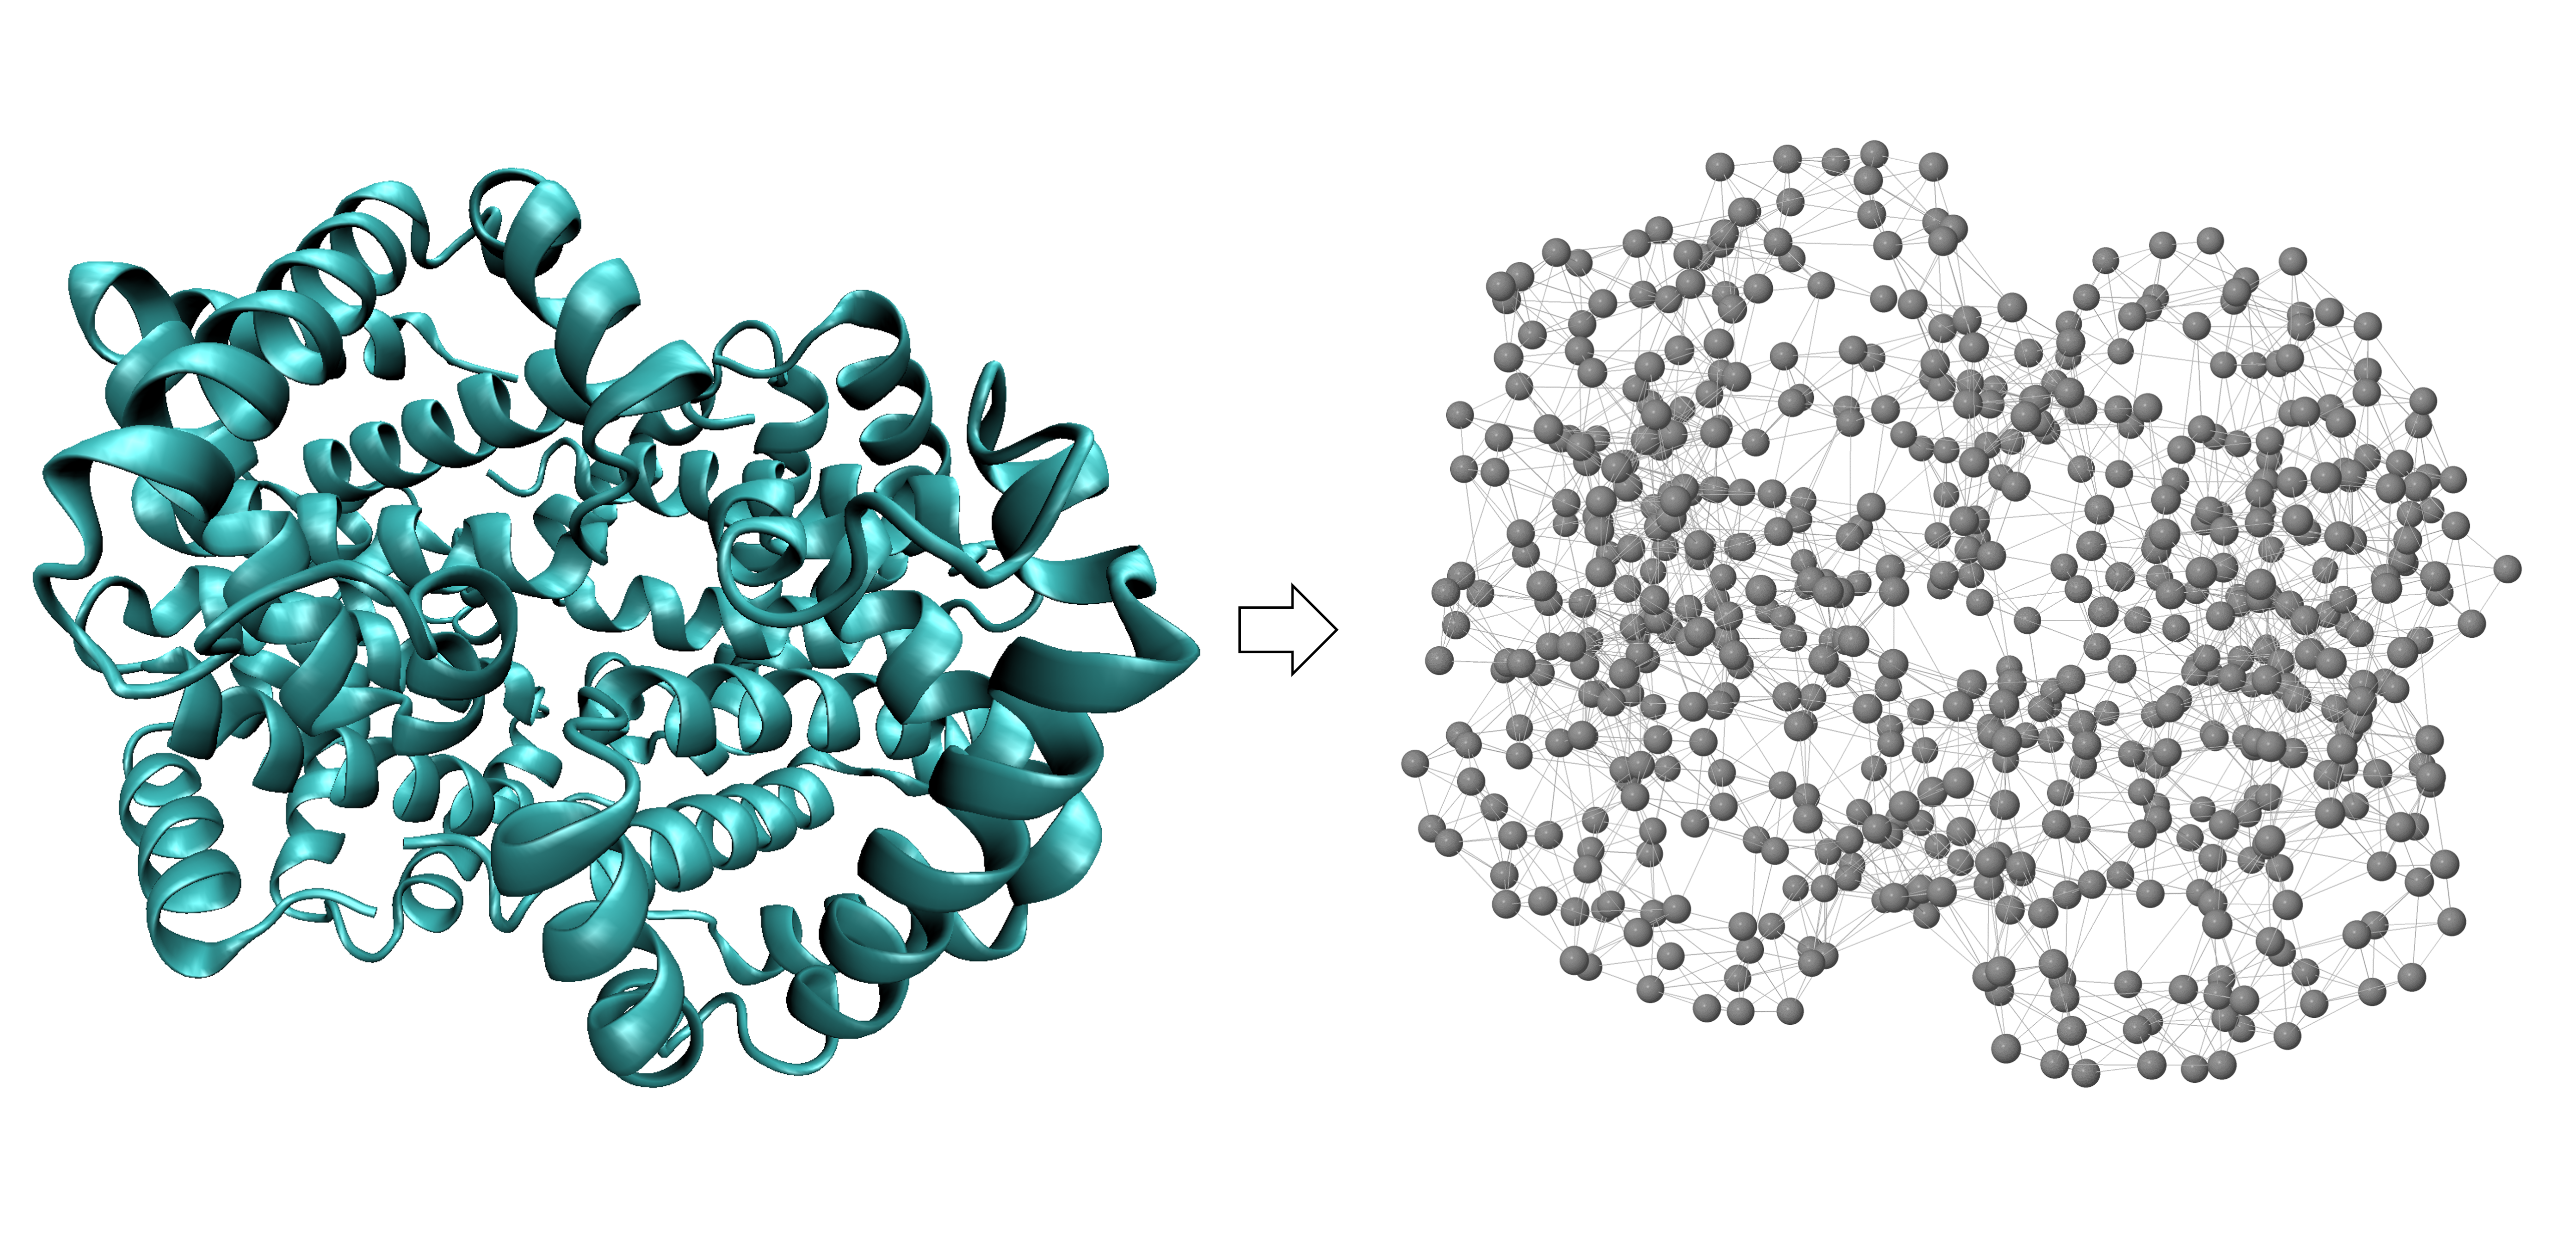
\includegraphics[width = 0.7\textwidth]{../images/hemoglobin_enm.png}
	\caption{Conversion of human hemoglobin (left) to a network of nodes and springs (right) in which two nodes are connected by a spring if they are within a threshold distance of 7.3 angstroms.}
	\label{fig:hemoglobin_enm}
\end{figure}

The alpha carbons in a protein are subject to random fluctuations that cause them to deviate from their equilibrium positions. These fluctuations are \textit{Gaussian}, which give the model its name. Gaussian fluctuations mean that the alpha carbon can deviate randomly from its equilibrium position according to a normal (bell-shaped) distribution, meaning that it is more likely to be near the equilibrium than far away.

The equilibrium position of node \textvar{i} is represented by the vector $\mathbf{R_i^0}$, and its position at a given point in time is denoted by the (variable) vector $ \mathbf{\Delta R_i}$. The distance between node \textvar{i} and node \textvar{j} at equilibrium is denoted by the vector $\mathbf{R_{ij}^0}$, which is equal to $\mathbf{R_j^0} - \mathbf{R_i^0}$ (as illustrated in \autoref{fig:gaussian_fluctuations}); at a given point in time, this distance becomes the vector $\mathbf{R_{ij}}$.

\begin{figure}[h]
	\centering
	\mySfFamily
	\includegraphics[width = 0.7\textwidth]{../images/gaussian_fluctuations.png}
	\caption{(Left) A small network of nodes connected by springs deriving from a protein structure. The distance between two nodes \textvar{i} and \textvar{j} is denoted by the variable $\textbf{R}_\textbf{ij}$. (Right) Zooming in on two nodes \textvar{i} and \textvar{j} that are within the threshold distance. The equilibrium positions of node \textvar{i} and node \textvar{j} are represented by the distance vectors $ \textbf{R}_\textbf{i}^\textbf{0} $ and $\textbf{R}_\textbf{j}^\textbf{0}$, with the distance between them denoted $\textbf{R}_{\textbf{ij}}^\textbf{0}$, which is equal to $\textbf{R}_\textbf{j}^\textbf{0} - \textbf{R}_\textbf{i}^\textbf{0}$. The vectors $\mathbf{\Delta} \textbf{R}_\textbf{i} $ and $ \mathbf{\Delta} \textbf{R}_\textbf{j}$ represent the nodes' respective changes from equilibrium.}
	\label{fig:gaussian_fluctuations}
\end{figure}

Yet although atomic fluctuations are powered by randomness, the movements of protein atoms are in fact heavily correlated. For example, imagine the simple case in which all of a protein's alpha carbons are connected in a straight line. If we pull the first alpha carbon away from the second node, then the second alpha carbon will be pulled toward the first alpha carbon, and the movements of these two alpha carbons will be directly correlated. Our goal is to understand how the movements of \textit{every} pair of alpha carbons, called the \textdefnogloss{cross-correlation} of these atoms, may be related. We will see how using vectors to represent these movements can be helpful.

\FloatBarrier
\phantomsection
\subsubsection{Inner products and cross-correlations}

To determine how the movements of nodes \textvar{i} and \textvar{j} are related, we need to study the fluctuation vectors $ \mathbf{\Delta R_i} $ and $\mathbf{\Delta R_j}$. Do these vectors point in similar or opposing directions?

To answer this question, we compute the \textdefnogloss{inner product}, or \textdefnogloss{dot product}, of the two vectors, $ \langle \mathbf{\Delta R_i}, \mathbf{\Delta R_j} \rangle $. The inner product of two vectors $\mathbf{x} = (x_1, x_2, x_3)$ and $\mathbf{y} = (y_1, y_2, y_3)$ is given by $ \langle \mathbf{x}, \mathbf{y} \rangle = x_1 \cdot y_1 + x_2 \cdot y_2 + x_3 \cdot y_3$. If $\mathbf{x}$ and $\mathbf{y}$ are perpendicular, then $ \langle \mathbf{x}, \mathbf{y} \rangle $ is equal to zero. The more that the two vectors point in the same direction, the larger the value of $\langle \mathbf{x}, \mathbf{y} \rangle $. And the more that the two vectors point in opposite directions, the smaller the value of $\langle \mathbf{x}, \mathbf{y} \rangle $.\\

\begin{qbox}[%
	Say that $\mathbf{x} = (1, -2, 3)$, $\mathbf{y} = (2, -3, 5)$, and  $\mathbf{z} = (-1, 3, -4)$. Compute the inner products $\langle \mathbf{x}, \mathbf{y} \rangle$ and $\langle \mathbf{x}, \mathbf{z} \rangle$  and ensure that your answers match the preceding observation.
	]\end{qbox}

The inner product is also useful for representing  the \textdefnogloss{mean-square fluctuation} of an alpha carbon, or the expected squared distance of node \textvar{i} from equilibrium. The fluctuation of node \textvar{i} from equilibrium is just $\mathbf{\Delta R_i}$. If this vector is represented by the coordinates (\textvar{x}, \textvar{y}, \textvar{z}), then its square distance from equilibrium is $x^2 + y^2 + z^2$, which is the inner product of the fluctuation vector with itself, $ \langle \mathbf{\Delta R_i}, \mathbf{\Delta R_i} \rangle $.\\

\begin{note}[%
	In practice, we will not know the exact values for the $ \mathbf{\Delta R_i} $ and must compute the inner products of fluctuation vectors indirectly using linear algebra, which is beyond the scope of this work. A full treatment of the mathematics of GNMs can be found in the chapter at \url{https://www.csb.pitt.edu/Faculty/bahar/publications/b14.pdf}.
	]\end{note}

Long vectors pointing in the same direction will have a larger inner product than short vectors pointing in the same direction. As a result, we can normalize the inner product so that we can have a sense of the correlation of these vectors, independent of their length. To be precise, the cross-correlation of nodes \textvar{i} and \textvar{j} is given by

\begin{center}
$ C_{ij} = \dfrac{\langle \mathbf{\Delta R_i}, \mathbf{\Delta R_i} \rangle}{\sqrt{\langle \mathbf{\Delta R_i}, \mathbf{\Delta R_i} \rangle \langle \mathbf{\Delta R_i}, \mathbf{\Delta R_i} \rangle}}$\,.
\end{center}

After normalization, the cross-correlation ranges from -1 to 1. A cross-correlation of -1 means that the two alpha carbons' movements are completely anti-correlated, and a cross-correlation of 1 means that their movements are completely correlated.

After computing the cross-correlation of every pair of alpha carbons in a protein structure with \textvar{n} residues, we obtain an $\textvar{n} \times \textvar{n}$ \textdefnogloss{cross-correlation matrix} \textvar{C} such that \textvar{C}(\textvar{i}, \textvar{j}) is the cross-correlation between amino acids \textvar{i} and \textvar{j}. We can visualize this matrix using a \textdefnogloss{heat map}, in which we color matrix values along a spectrum from blue ($-1$) to red (1). The heat map for the cross-correlation matrix of human hemoglobin is shown in \autoref{fig:hemoglobin_cc}.\\

\begin{figure}[h]
	\centering
	\mySfFamily
	\includegraphics[width = 0.6\textwidth]{../images/hemoglobin_cc.png}
	\caption{The normalized cross-correlation heat map of human hemoglobin (PDB: 1A3N). Red regions indicate correlated residue pairs which move in the same direction; blue regions indicate anti-correlated residue pairs which move in opposite directions. Note that the matrix is oriented so that its first element is in the bottom left corner.}
	\label{fig:hemoglobin_cc}
\end{figure}

The cross-correlation map of a protein contains complex patterns of correlated and anti-correlated movement of the protein's atoms. Much like the contact map that we showed in an earlier section, it serves as a ``fingerprint'' of sorts for the protein and can give useful insights into the protein's structure.

For example, we should not be surprised that the main diagonal of the cross-correlation map is colored red, since alpha carbons that are near each other in a polypeptide chain will likely have correlated movements.

Furthermore, the regions of high correlation near the main diagonal typically provide information regarding the protein's secondary structures, since amino acids belonging to the same secondary structure will typically move in concert.

High correlation regions that are far away from the matrix's main diagonal provide information about the \textit{tertiary} structure of the protein, such as protein domains and other components of the protein that work together.

Consider again the cross-correlation map of human hemoglobin in \autoref{fig:hemoglobin_cc}. We can see four squares of positive correlation along the main diagonal, representing the four subunits of hemoglobin from bottom left to top right: $\alpha_1$, $\beta_1$, $\alpha_2$, and $\beta_2$. Note that the first and third squares have the same patterns; these squares correspond to $\alpha_1$ and $\alpha_2$, respectively. Similarly, the second and fourth squares correspond to $\beta_1$ and $\beta_2$.\\

\begin{qbox}[%
	What other patterns do you notice in the hemoglobin cross-correlation heat map?
	]\end{qbox}

\FloatBarrier
\phantomsection
\subsubsection{Mean-square fluctuations and B-factors}

Just as we can visualize cross-correlation, we could also plot the mean-square fluctuations of residues using a line graph, where the x-axis represents the order of alpha carbons, and the y-axis represents the mean-square fluctuation $ \langle \mathbf{\Delta R_i}, \mathbf{\Delta R_i} \rangle $ of the \textvar{i}-th alpha carbon. Large \textvar{y}-values in this plot would correspond to mobile alpha carbons, whereas lower values would correspond to static alpha carbons.

We also would like to compare these predicted mean-square fluctuations against what we can infer from experimental results. During X-ray crystallography, the displacement of atoms within the protein crystal decreases the intensity of the scattered X-ray, creating uncertainty in the positions of atoms. \textdefnogloss{B-factor}, also known as \textbf{temperature factor} or \textbf{Debye-Waller factor}, is a measure of this uncertainty, which includes noise from positional variance of thermal protein motion, model errors, and lattice defects.

We can then compare these \textit{experimental} B-factors against a \textit{theoretical} estimate of their value. It is beyond the scope of this work, but the theoretical B-factors are given by

\begin{center}
$ B_i = \dfrac{8 \pi^2}{3} \langle \mathbf{\Delta R_i}, \mathbf{\Delta R_i} \rangle$\,.
\end{center}

In other words, once we can estimate the mean-square fluctuations $\langle \mathbf{\Delta R_i}, \mathbf{\Delta R_i} \rangle$, the theoretical B-factor of the \textvar{i}-th alpha carbon is equal to a constant times this inner product. This theoretical B-factor tends to correlate well with theoretical B-factors in practice.

\autoref{fig:hemoglobin_b_factors} shows a plot of the B-factor of the α\textsubscript{1} subunit of human hemoglobin. We also show a 3-D structure of the hemoglobin protein, with amino acids colored along a spectrum according to both theoretical and experimental B-factors for the sake of comparison. In these structures, red indicates large B-factors (mobile amino acids), and blue indicates small B-factors (static amino acids). Note that the mobile amino acids are generally found at the ends of secondary structures in the outer edges of the protein, which is expected because the boundaries between secondary structures typically contain highly fluctuating residues.\\

\begin{figure}[h]
	\centering
	\mySfFamily
	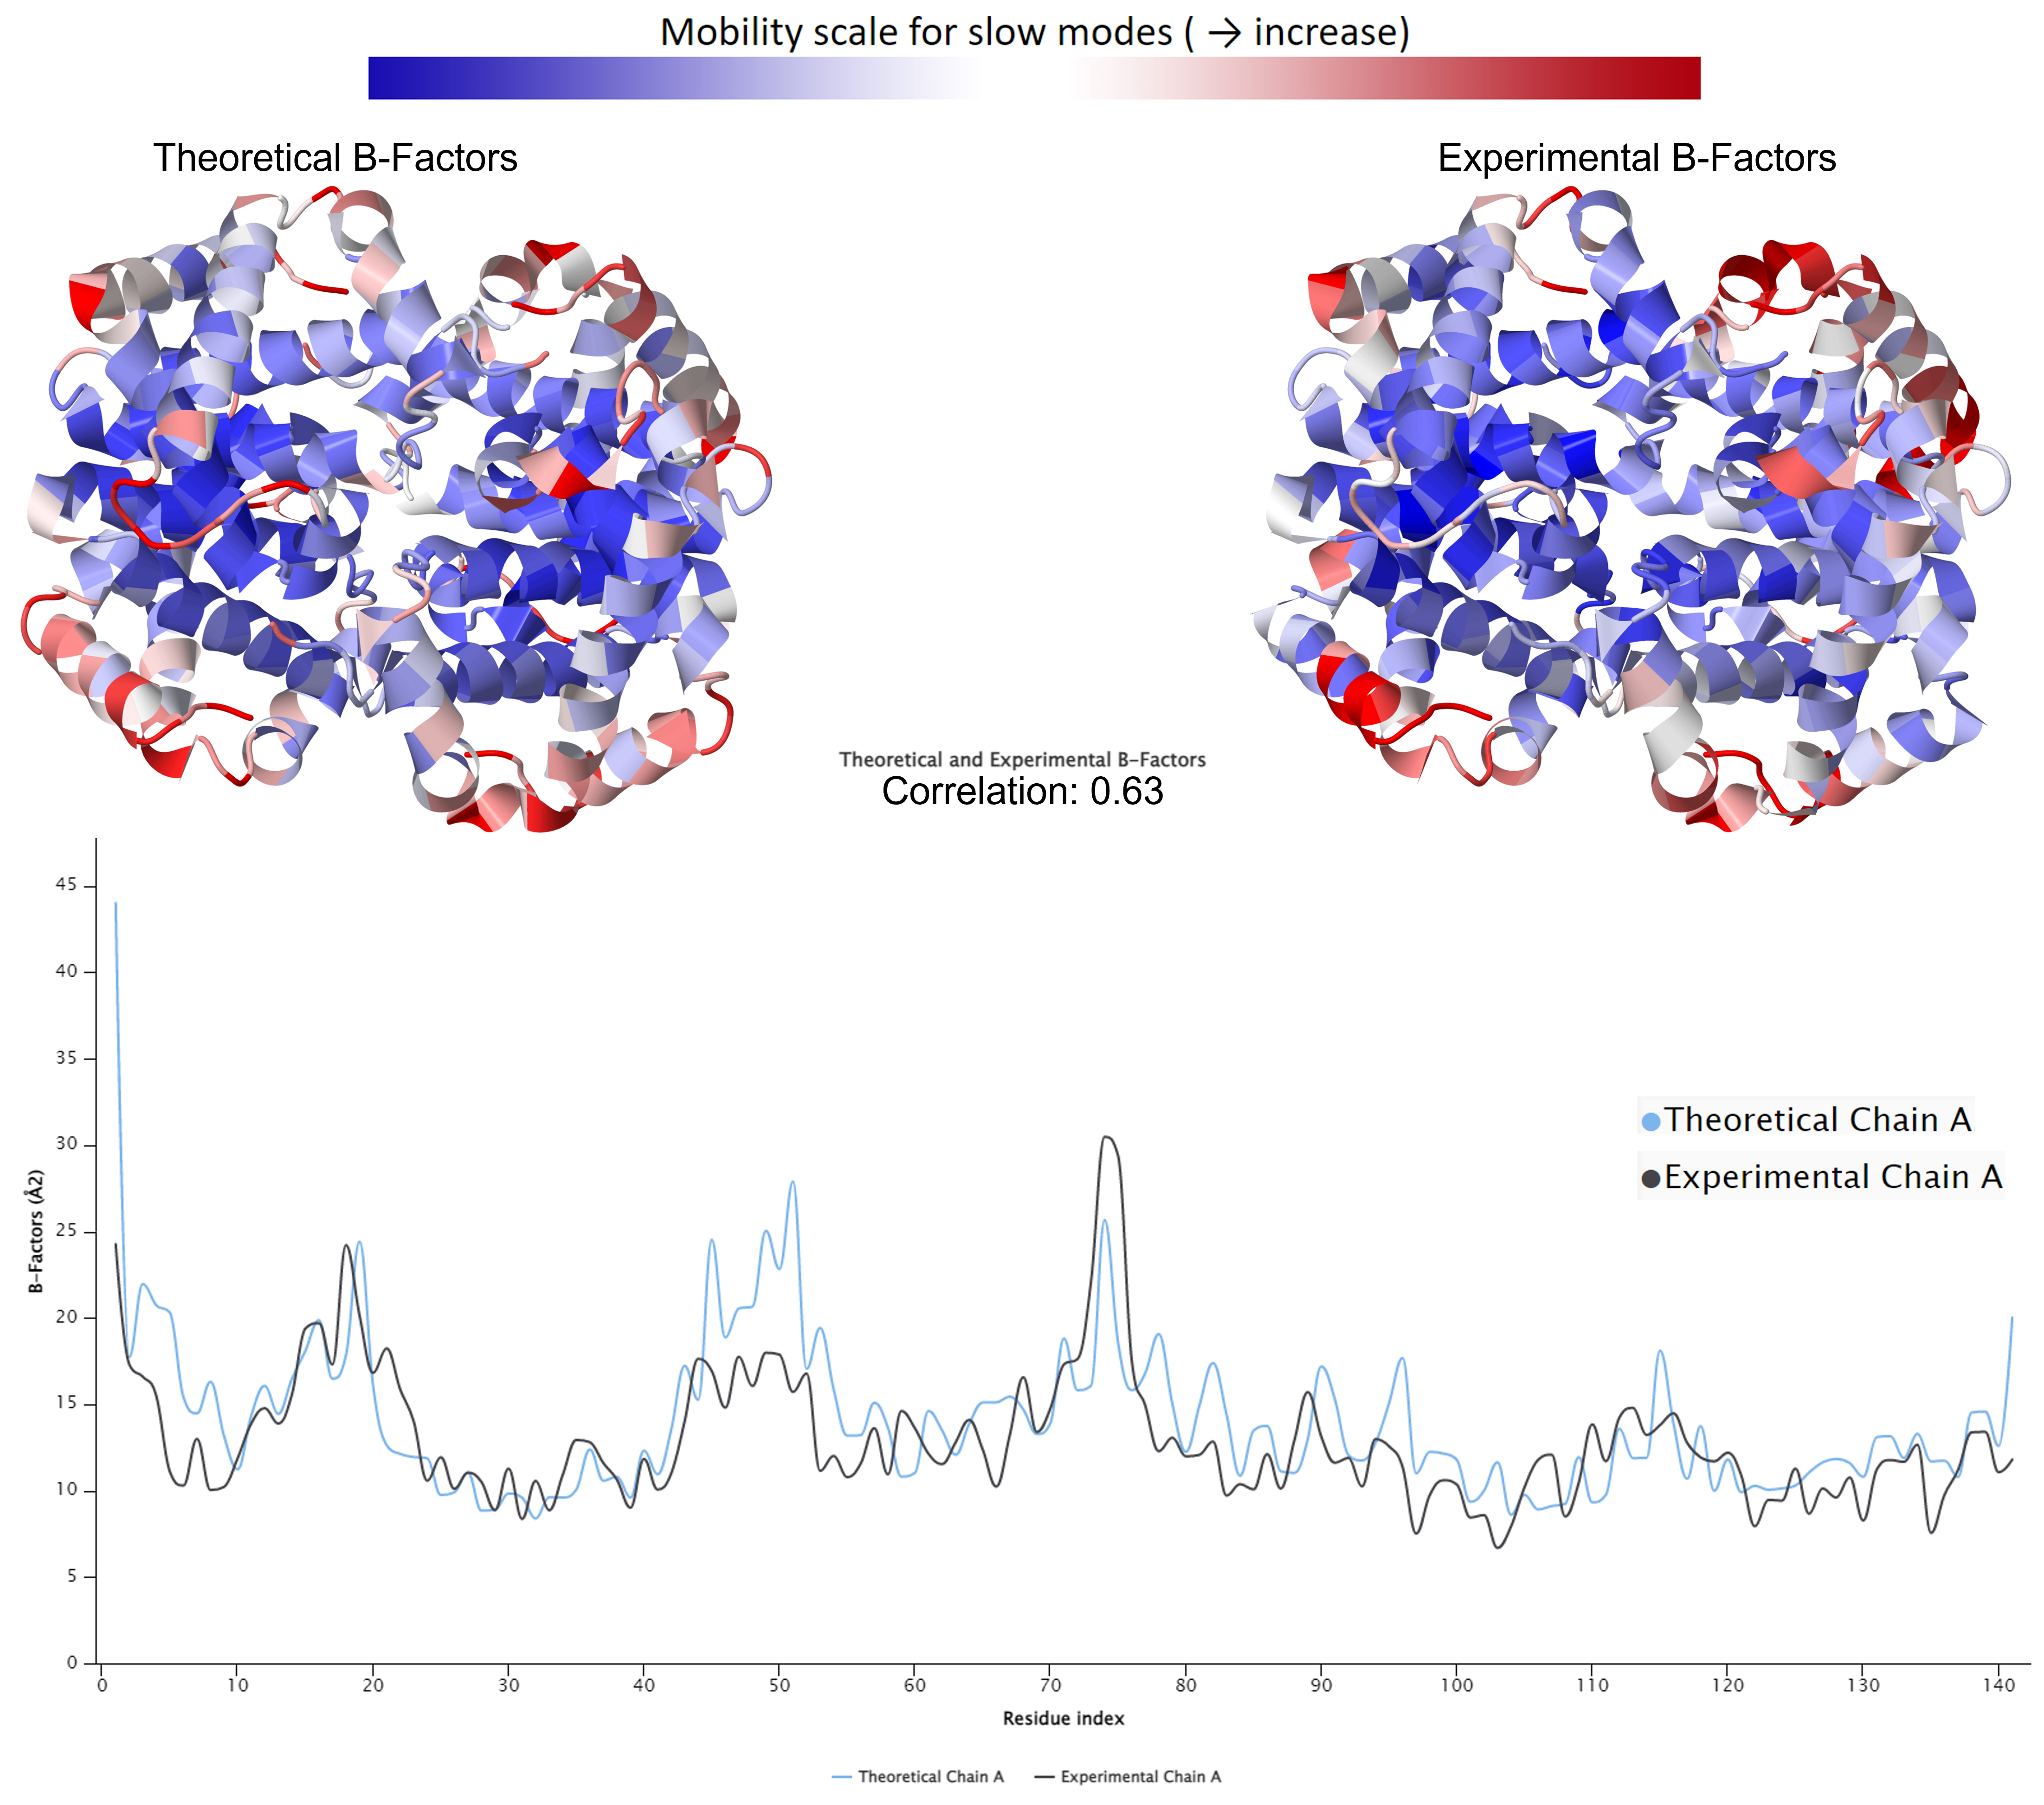
\includegraphics[width = 0.85\textwidth]{../images/hemoglobin_b_factors.png}
	\caption{(Top): Human hemoglobin colored according to theoretical B-factors calculated from GNM (left) and experimental B-factors (right). Subunit $\text{α}_\text{1}$ is located at the top left quarter of the protein figure. (Bottom): A 2-D plot comparing the theoretical (blue) and experimental (black) B-factors of subunit $\text{α}_\text{1}$.  The theoretical and experimental B-factors are correlated with a coefficient of 0.63.}
	\label{fig:hemoglobin_b_factors}
\end{figure}

\FloatBarrier
\phantomsection
\subsection{Normal mode analysis}

When listening to your favorite song, you probably do not think of the individual notes that it comprises. Yet a talented musician can dissect the song into the set of notes that each instrument contributes to the whole. Just because the music combines a number of individual sound waves does not mean that we cannot deconvolve the music into its substituent waves.

All objects, from colossal skyscrapers to tiny proteins, vibrate. And, just like in our musical example, these oscillations are the net result of individual waves passing through the object. The paradigm of breaking down a collection of vibrations into the comparatively small number of ``modes'' that summarize them is called \textdef{normal mode analysis (NMA)}{normal mode analysis (NMA)}{the paradigm of breaking down a collection of vibrations into the comparatively small number of ``modes'' that summarize them} and is at the heart of elastic network models.

The mathematical details are complicated, but by deconvolving a protein's movement into individual normal modes, we can observe how each mode affects individual amino acids. As we did with B-factors, for a given mode, we can visualize the results of a mode with a line graph, called the \textdefnogloss{mode shape plot}. The x-axis of this plot corresponds to the amino acid sequence of the protein, and the height of the \textvar{i}-th position on the x-axis corresponds to the magnitude of the square fluctuation caused by the mode on the protein's \textvar{i}-th residue.

Just as a piece of music can have one instrument that is much louder than another, some of the oscillations contributing to an object's vibrations may be more significant than others. NMA also determines the degree to which each mode contributes to the overall fluctuations of a protein; the mode contributing the most is called the \textdefnogloss{slowest mode} of the protein. \autoref{fig:hemoglobin_mode_shape} shows a mode shape plot of the slowest mode for each of the four subunits of human hemoglobin.

\begin{figure}[h]
	\centering
	\mySfFamily
	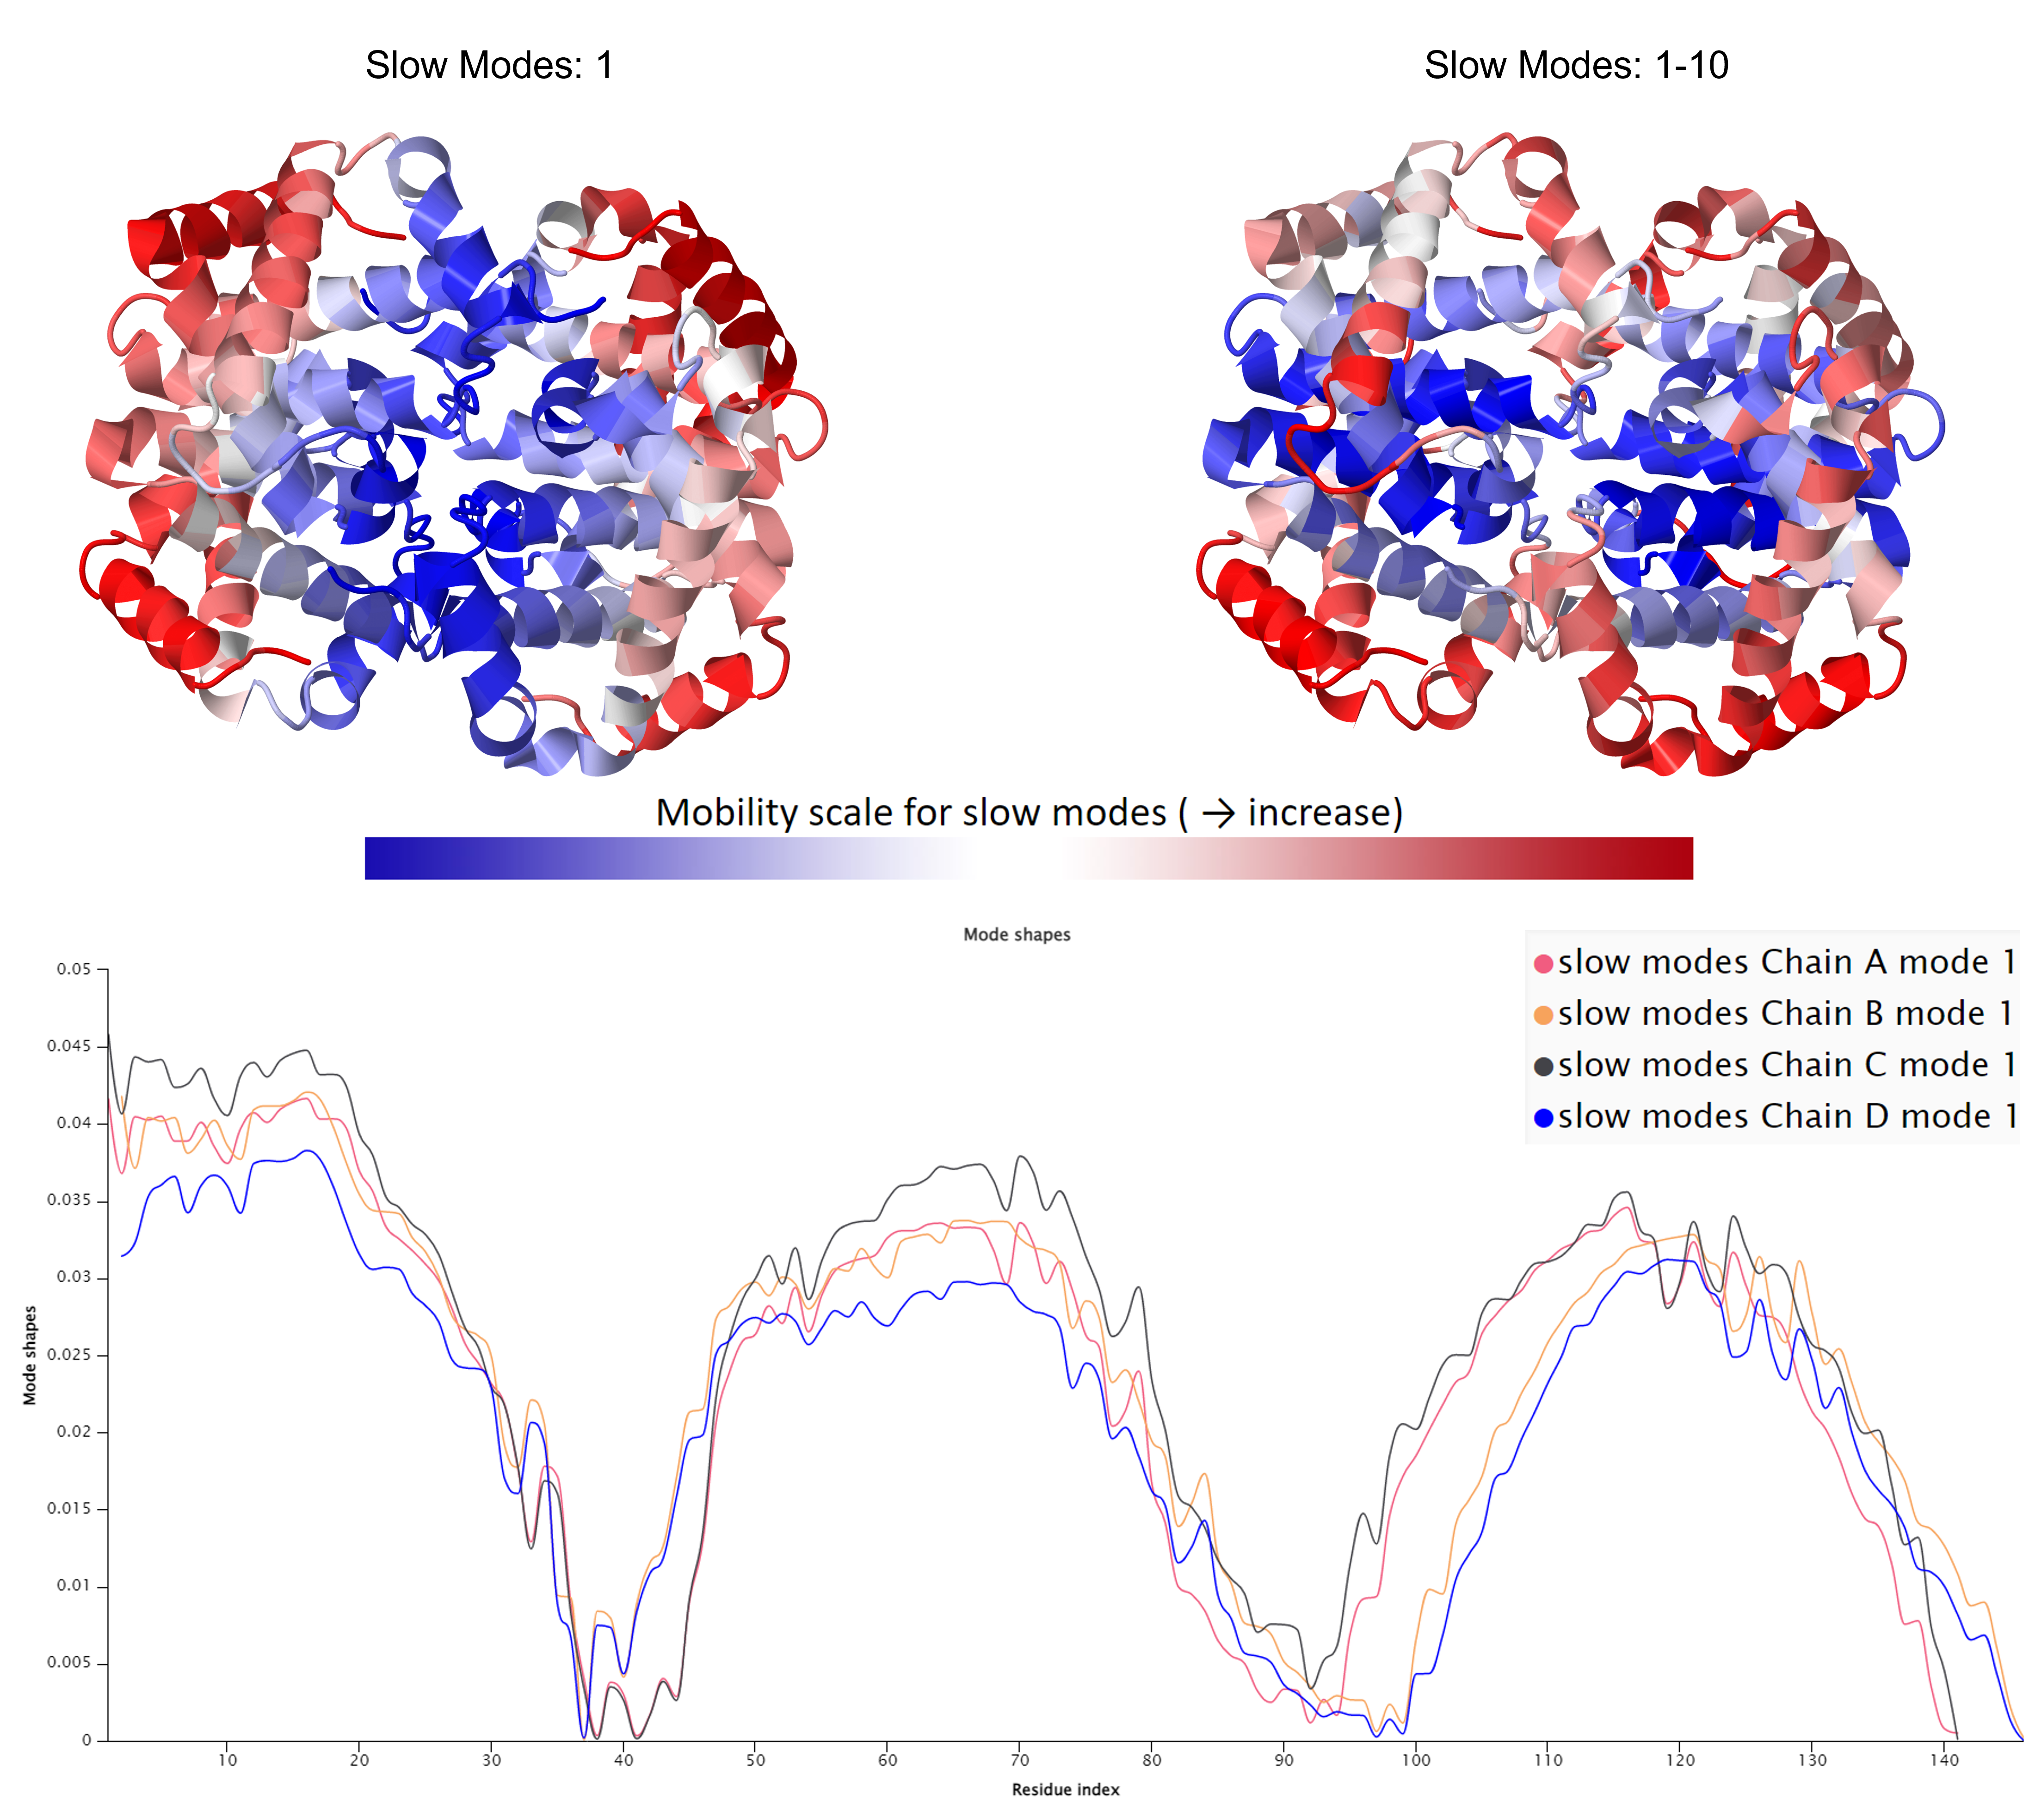
\includegraphics[width = 0.7\textwidth]{../images/hemoglobin_mode_shape.png}
	\caption{(Top) Visualization of human hemoglobin colored based on GNM slow mode shape for the slowest mode (left) and the average of the ten slowest modes (right), or the ten modes that contribute the most to the square fluctuation. Regions of high mobility are colored red, corresponding to peaks in the mode shape plot. (Bottom) A mode shape plot of the slowest mode for human hemoglobin, separated over each of the four chains, shows that the four chains have a similar slowest mode.}
	\label{fig:hemoglobin_mode_shape}
\end{figure}

Similar to cross-correlation, analyzing a protein's mode shapes will give insights into the structure of the protein, and comparing mode shapes for two proteins can reveal structural differences. For example, the mode shape plots in \autoref{fig:hemoglobin_mode_shape} show that the slowest mode shape for the four subunits of hemoglobin are quite similar.

We should consult more than just a single mode when completing a full analysis of a protein's molecular dynamics. \autoref{fig:hemoglobin_mode_shape_avg} is the slow mode plot averaging the ``slowest'' ten modes of hemoglobin, meaning the modes that have the greatest affect on mean fluctuation. Unlike when we examined only the slowest mode, we can now see a stark difference between the two groups of subunits/chains; the plots for $\alpha$ subunits (chains A and C) are very similar, whereas the plots for $\beta$ subunits (chains B and D) share a slightly less similar average slow mode shape.\\

\begin{figure}[h]
	\centering
	\mySfFamily
	\includegraphics[width = 0.85\textwidth]{../images/hemoglobin_mode_shape_avg.png}
	\caption{The average mode shape of the slowest ten modes for each of the four human hemoglobin subunits using GNM.}
	\label{fig:hemoglobin_mode_shape_avg}
\end{figure}

We are now ready to apply what we have learned in this section and use ProDy to build a GNM for the SARS-CoV and SARS-CoV-2 spike proteins. \tutorial[coronavirus/tutorial_GNM]

\FloatBarrier
\phantomsection
\subsection{Molecular dynamics analyses of SARS-CoV and SARS-CoV-2 spike proteins using GNM}

\autoref{fig:CrossCorr} shows the cross-correlation heat maps of SARS-CoV and SARS-CoV-2 spike proteins, indicating that these proteins may have similar dynamics.\\

\begin{figure}[h]
	\centering
	\mySfFamily
	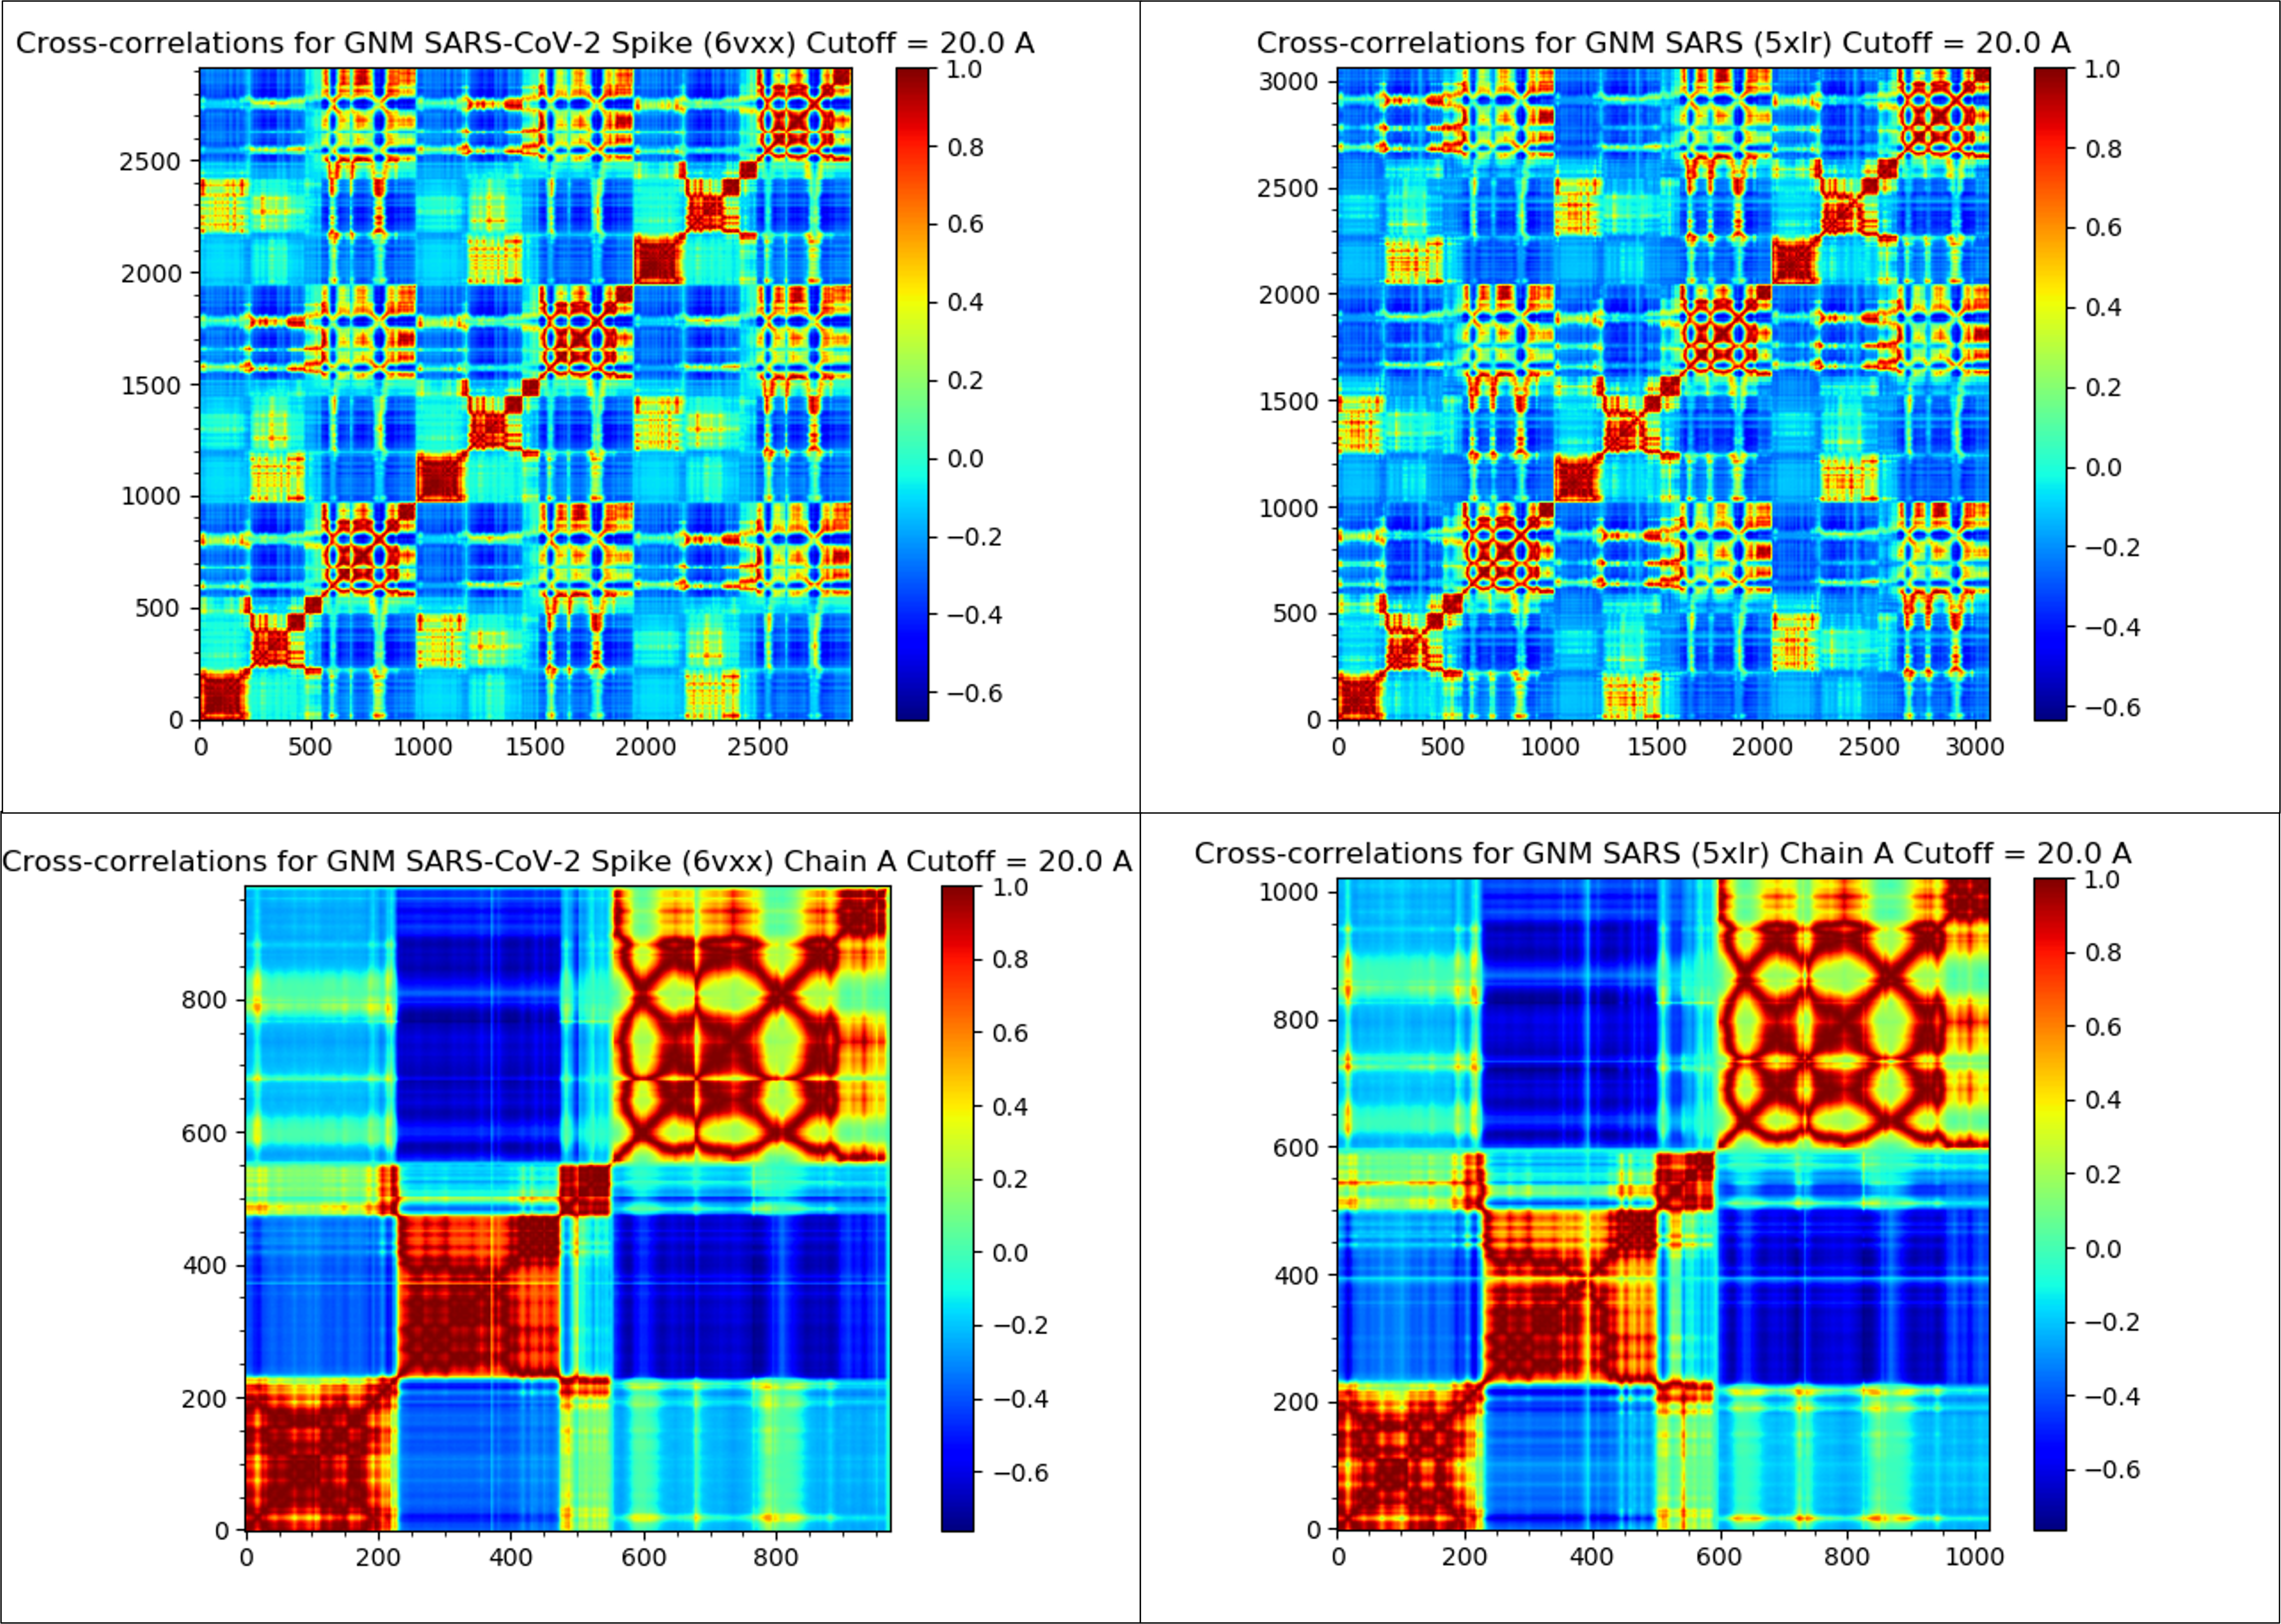
\includegraphics[width = 0.85\textwidth]{../images/CrossCorr.png}
	\caption{The cross-correlation heat maps of the SARS-CoV-2 spike protein (top-left), SARS-CoV spike protein (top-right), single chain of the SARS-CoV-2 spike protein (bottom-left), and single-chain of the SARS-CoV spike protein (bottom-right).}
	\label{fig:CrossCorr}
\end{figure}

\autoref{fig:SlowMode} shows the mode shape plot for the slowest mode of the two proteins. The protein region between positions 200 and 500 of the spike protein is the most mobile and overlaps with the RBD region, found between residues 331 to 524.\\

\begin{figure}[h]
	\centering
	\mySfFamily
	\includegraphics[width = 0.85\textwidth]{../images/SlowMode.png}
	\caption{(Top) A mode shape plot for the slowest mode of the SARS-CoV-2 spike protein (left) and SARS-CoV spike protein (right). (Bottom) A mode shape plot for the slowest mode of a single chain of the SARS-CoV-2 spike protein (left) and a single chain of the SARS-CoV spike protein (right). Note that the plot on the right is inverted compared to the one on the left because of a choice made by the software, but the two plots have the same shape if we consider the absolute value. These plots show that the two viruses have similar dynamics, and that residues 200 to 500 fluctuate the most, a region that overlaps heavily with the RBD.}
	\label{fig:SlowMode}
\end{figure}

We can also examine the mode shape plot for the average of the slowest ten modes for the two spike proteins (\autoref{fig:spike_slowmode_comparison}). Using this plot, we color flexible parts of the protein red and inflexible parts of the protein blue.\\

\begin{figure}[h]
	\centering
	\mySfFamily
	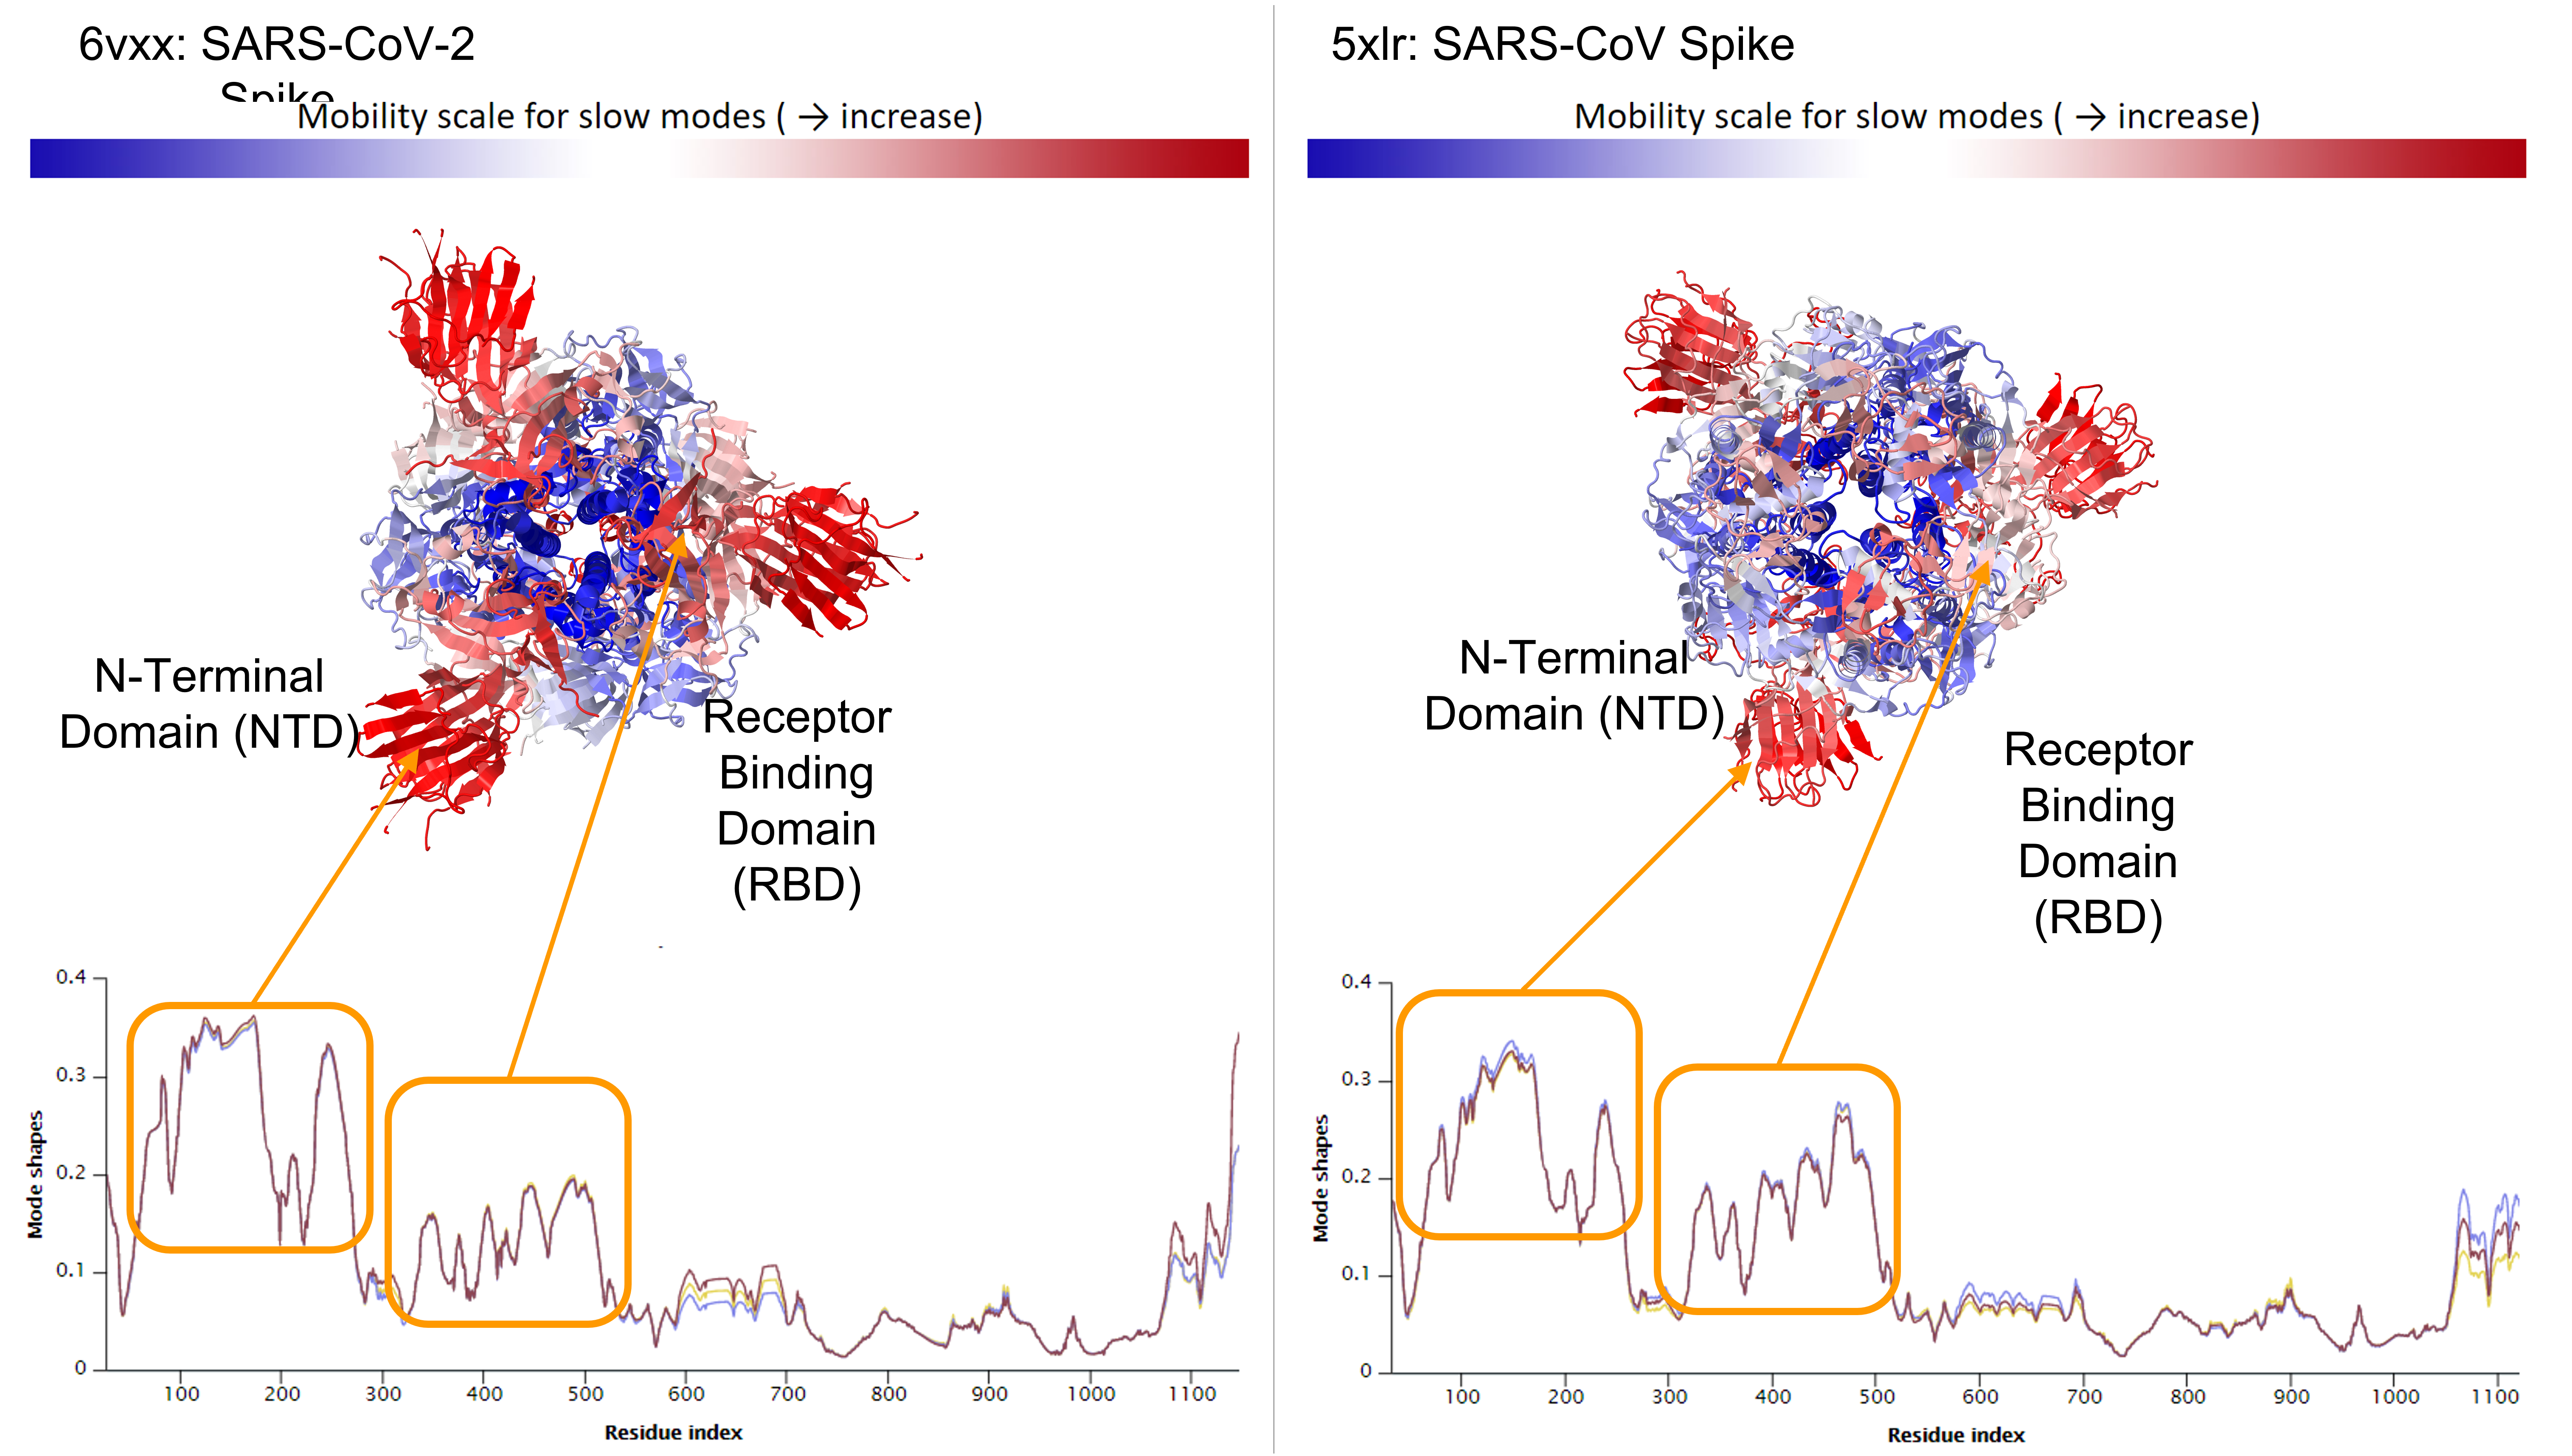
\includegraphics[width = 0.85\textwidth]{../images/spike_slowmode_comparison.png}
	\caption{Average mode shape of the slowest ten modes of SARS-CoV-2 Spike (left) and SARS-CoV Spike (right). The first peak corresponds to the N-Terminal Domain (NTD) and the second peak corresponds to the Receptor Binding Domain (RBD).}
	\label{fig:spike_slowmode_comparison}
\end{figure}

The mode shape plots show that the RBD of both spike proteins are highly flexible, which agrees with the biological functions of these regions. When the RBD interacts with the ACE2 enzyme on human cells, the RBD of one of the three chains ``opens up'', exposing itself to more easily bind with ACE2.

\autoref{fig:spike_slowmode_comparison} highlights another flexible region, the spike protein's \textdefnogloss{non-terminal domain (NTD)}. Similar to the RBD, the NTD of the Spike proteins also mediates viral infection, but by interacting with DC-SIGN and L-SIGN receptors rather than ACE2. These receptors are present on macrophages and dendritic cells, allowing SARS-CoV-2 to infect different tissues such as the lungs, where ACE2 expression levels are low. The ability to infect lung cells attributes to pneumonia, the main symptom of severe COVID-19 cases. As with the RBD, the high flexibility in this domain allows the spike protein to more easily interact with these receptors.

We should perhaps not be surprised that these plots point to SARS-CoV-2 and SARS-CoV having similar dynamics, since their structures were similar, and both viral proteins target the ACE2 enzyme. To help provide more evidence for their similarity, we will learn about another aspect of molecular dynamics.

\FloatBarrier
\phantomsection
\subsection{ANM accounts for the direction of protein fluctuations}

All of the analysis provided by GNM, from cross-correlation plots to B-factors and NMA, depend on the estimation of inner products $ \langle \mathbf{\Delta R_i}, \mathbf{\Delta R_i} \rangle $ or $ \langle \mathbf{\Delta R_i}, \mathbf{\Delta R_i} \rangle $ as the case may be. Although the $ \mathbf{\Delta R_i} $ are vectors, meaning that they have a \textvar{direction} as well as a magnitude, the inner products have only a value, and we therefore are not able to infer anything about the direction of a protein's movements. For this reason, GNM is said to be \textdefnogloss{isotropic}, meaning that it only considers the magnitude of force exerted on the springs between nearby molecules and ignores any global effect on the directions of these forces.

The generalization of GNM in which we attempt to determine the directions of these forces is called an \textdef{anisotropic network model (ANM)}{anisotropic network model (ANM)}{a generalization of a Gaussian network model accounting for the directions of the forces acting on atoms}. Although ANM includes directionality, it typically performs worse than GNM when compared with experimental data. However, this model offers the benefit that it can be used to create animations depicting the range of motions and fluctuations of the protein, as well as to estimate the directions of movement caused by each of a protein's modes.

We will not delve into the mathematical intricacies of ANM calculations, but we will use ANM to create animations visualizing protein fluctuations. For example, \autoref{fig:hemoglobin_anm_2} shows the estimated hemoglobin fluctuations produced from ANM. We can see that the left and right side of the protein are more flexible than the rest of the protein and twist in opposite directions.\\

\begin{figure}[h]
	\centering
	\tabcolsep = 1em
	\mySfFamily
	\begin{tabular}{c c c}
		\includegraphics[width = 0.25\textwidth]{../images/hemoglobin_animation1.png} & \includegraphics[width = 0.25\textwidth]{../images/hemoglobin_animation2.png} & \includegraphics[width = 0.25\textwidth]{../images/hemoglobin_animation3.png}
	\end{tabular}
	\caption{Collective motions of the slowest mode in human hemoglobin from ANM calculations using DynOmics.}
	\label{fig:hemoglobin_anm_2}
\end{figure}


After we produce an animation like the one in \autoref{fig:hemoglobin_anm_2}, we also should attempt to explain it biologically. Human hemoglobin exists in two states: the tense state (T), in which it is not bound to an oxygen molecule, and the relaxed state (R), in which it is oxygenated. Hemoglobin's mobility shown in the above animation corresponds to its ability to transition between these two states, in which salt-bridges and contacts can shift by up to seven angstroms. This significant molecular flexibility exemplifies why we need to study protein dynamics as well as structure.

We will now apply ANM to the SARS-CoV and SARS-CoV-2 spike proteins. We will also use \href{http://prody.csb.pitt.edu/nmwiz/}{\textdefnogloss{NMWiz}}, which is short for ``normal mode wizard'', to perform ANM calculations and create an animation of the SARS-CoV-2 (chimeric) RBD and the SARS-CoV RBD. \tutorial[coronavirus/tutorial_ANM]

\FloatBarrier
\phantomsection
\subsection{ANM accounts for the direction of protein fluctuations}

To predict spike protein movements based on ANM, we used NMWiz and VMD to create animations of the protein fluctuations over time as calculated via ANM analysis. \autoref{fig:2ajf_animation} and \autoref{fig:6vw1_animation} show the complex of each virus's RBD (purple) bound with ACE2 (green). Important residues from the three sites of conformational differences identified previously in this chapter are also highlighted.

\FloatBarrier
\phantomsection
\subsection{SARS-CoV spike protein RBD (PDB: 2ajf)}

\begin{figure}[h]
	\centering
	\tabcolsep = 1 em
	\mySfFamily
	\begin{tabular}{c c }
		\textbf{SARS-CoV RBD} & \textbf{Purple} \\
		Resid 463 to 472 (Loop)  & Yellow \\
		Resid 442 (Hotspot 31)  & Orange \\
		Resid 487 (Hotspot 353)  & Red \\
		\textbf{ACE2}  & \textbf{Green} \\
		Resid 79, 82, 83 (Loop) & Silver \\
		Resid 31, 35 (Hotspot 31) & Orange \\
		Resid 38, 353 (Hotspot 353) & Red \\
	\end{tabular}
	\caption{}
	\label{fig:2ajf_B&F_table}
\end{figure}

\begin{figure}[h]
	\centering
	\tabcolsep = 1em
	\mySfFamily
	\begin{tabular}{c c c}
		\includegraphics[width = 0.25\textwidth]{../images/2ajf_animation1.png} & \includegraphics[width = 0.25\textwidth]{../images/2ajf_animation2.png} & \includegraphics[width = 0.25\textwidth]{../images/2ajf_animation3.png}
	\end{tabular}
	\caption{Snapshots of ANM analysis animation of SARS-CoV-2 spike RBD and ACE2 (PDB entry: 2ajf)}
	\label{fig:2ajf_animation}
\end{figure}

\FloatBarrier
\phantomsection
\subsection{SARS-CoV-2 spike protein chimeric RBD (PDB: 6vw1)}

\begin{figure}[h]
	\centering
	\tabcolsep = 1 em
	\mySfFamily
	\begin{tabular}{c c }
		\textbf{SARS-CoV-2 (Chimeric) RBD} & \textbf{Purple} \\
		Resid 476 to 486 (Loop)  & Yellow \\
		Resid 455 (Hotspot 31)  & Blue \\
		Resid 493 (Hotspot 31) & Orange \\
		Resid 501 (Hotspot 353) & Red \\
		\textbf{ACE2}  & \textbf{Green} \\
		Resid 79, 82, 83 (Loop) & Silver \\
		Resid 31, 35 (Hotspot 31) & Orange \\
		Resid 38, 353 (Hotspot 353) & Red \\
	\end{tabular}
	\caption{}
	\label{fig:6vw1_B&F_table}
\end{figure}

\begin{figure}[h]
	\centering
	\tabcolsep = 1em
	\mySfFamily
	\begin{tabular}{c c c}
		\includegraphics[width = 0.25\textwidth]{../images/6vw1_animation1.png} & \includegraphics[width = 0.25\textwidth]{../images/6vw1_animation2.png} & \includegraphics[width = 0.25\textwidth]{../images/6vw1_animation3.png}
	\end{tabular}
	\caption{Snapshots of ANM analysis animation of SARS-CoV-2 spike chimeric RBD and ACE2 (PDB entry: 6vw1)}
	\label{fig:6vw1_animation}
\end{figure}

Recall from \autoref{sec:interaction_energy} that the greatest contribution of negative energy to the RBD/ACE2 complex in SARS-CoV-2 was the region called ``hotspot 31''. This region is highlighted in blue and orange in \autoref{fig:6vw1_animation}. If you look very closely, as the protein swings in to bind with ACE2, the blue and orange regions appear to line up just a bit more naturally in the SARS-CoV-2 animation than in the SARS-CoV animation. That is, the improved binding that we hypothesized for a static structure appears to be confirmed by dynamics simulations. This animation provides one more piece of evidence that SARS-CoV-2 is more effective at binding to the ACE2 enzyme.

\FloatBarrier
\phantomsection
\subsection{DynOmics Integrates GNM and ANM Analysis}

Although we have separated our discussion of GNM and ANM, the DynOmics 1.0 server (\url{http://enm.pitt.edu/index.php}) is an effort to integrate these approaches on a user-friendly platform. \tutorial[coronavirus/tutorial_DynOmics]

\FloatBarrier
\phantomsection
\subsection{Fighting a Virus with Open Science}

In this chapter, we began with a discussion of the fundamental problem of determining a protein's structure. Because experimental methods for identifying protein structure are costly and time consuming, we transitioned to discuss algorithmic approaches that do a good job of predicting a protein's structure from its sequence of amino acids.

We then discussed how to compare protein structures, with a lengthy case study comparing the SARS-CoV and SARS-CoV-2 spike proteins. The problem of quantifying how different two structures is can be challenging, and we established both global and local structure comparison metrics. We applied these approaches to isolate three candidate regions of interest of the SARS-CoV-2 spike protein that differ from the SARS-CoV spike protein when complexed with the ACE2 enzyme, and we quantified this binding using a localized energy function.

We concluded with a transition from the study of structure to the structure of molecular dynamics. If we hope to fully understand a protein's function, then we need to know how it flexes and bends within its environment, sometimes in order to interact with other molecules.

Despite covering a great deal of ground, we have left just as much unstudied. For one example, the surface of viruses and host cells are ``fuzzy'' because they are covered by structures called \textdef{glycans}{glycans}{numerous monosaccharides linked together on the surface of viruses and host cells}, or numerous monosaccharides linked together. SARS-CoV and SARS-CoV-2 have a “glycan shield”, in which glycosylation of surface antigens allows the virus to hide from antibody detection. Researchers have found that the SARS-CoV-2 spike protein is heavily glycosylated, shielding around 40\% of the protein from antibody recognition; we will save a comparative analysis of the two virus's glycan shields for another time.

Finally, we would point out that although scientific research has often historically been siloed away from the public, the COVID-19 pandemic exemplifies how global citizens can get involved in real research. \href{https://www.gisaid.org}{GISAID} published their first publicly available SARS-CoV-2 genome on December 24, 2019. Within six months, this database had grown to contain over 50,000 entries, and after two years, it would contain nearly 7 million.

At any point in early 2020, you could have grabbed your favorite SARS-CoV-2 genome sequenced from a patient, excised the sequence of the spike protein, and used one of a variety of different software resources to predict its structure. Or, you could have enlisted your own computer as part of a global race to provide vaccine developers with accurate estimations of the protein's structure. Despite the COVID-19 pandemic causing an international crisis, the progress made in opening scientific research to the public is cause for optimism about the future of biological research.

Thus concludes our discussion of protein analysis. In \autoref{chapter:white_blood_cells}, we will turn our attention to a very different type of problem. To fight a virus like SARS-CoV-2, your body employs a cavalry of white blood cells. Maintaining healthy levels of these cells is vital to a strong immune system, and blood reports run counts of these cells to ensure they are within normal ranges. Can we teach a computer to run this analysis automatically?\\

\FloatBarrier
\section{Exercises}
\label{sec:coronavirus_exercises}
\phantomsection

\begin{exercise}[%
	Test of exercise environment.
	]\end{exercise}
